%\pdfoutput=1
% Uncomment line above if submitting to arXiv and using pdflatex

% $Id: main.tex 87005 2016-02-02 15:50:33Z siborghi $
% ============================================================================
% Purpose: Template for LHCb documents
% Authors: Tomasz Skwarnicki, Roger Forty, Ulrik Egede
% Created on: 2010-09-24
% ============================================================================
\documentclass[12pt,a4paper]{article}
% For two column text, add "twocolumn" as an option to the document
% class. Also uncomment the two "onecolumn" and "twocolumn" lines
% around the title page below.

% Variables that controls behaviour
\usepackage{ifthen} % for conditional statements
\newboolean{pdflatex}
\setboolean{pdflatex}{true} % False for eps figures 

\newboolean{articletitles}
\setboolean{articletitles}{true} % False removes titles in references

\newboolean{uprightparticles}
\setboolean{uprightparticles}{false} %True for upright particle symbols

\newboolean{inbibliography}
\setboolean{inbibliography}{false} %True once you enter the bibliography

% THis file contains all the default packages and modifications for
% LHCb formatting

%% %%%%%%%%%%%%%%%%%%
%%  Page formatting
%% %%%%%%%%%%%%%%%%%%
\textheight=230mm
\textwidth=160mm
\oddsidemargin=7mm
\evensidemargin=-10mm
\topmargin=-10mm
\headsep=20mm
\columnsep=5mm
\addtolength{\belowcaptionskip}{0.5em}

\renewcommand{\textfraction}{0.01}
\renewcommand{\floatpagefraction}{0.99}
\renewcommand{\topfraction}{0.9}
\renewcommand{\bottomfraction}{0.9}


\setlength{\hoffset}{-2cm}
\setlength{\voffset}{-2cm}
% Page defaults ...
\topmargin=0.5cm
\oddsidemargin=2.5cm
\textwidth=16cm
\textheight=22cm
% Allow the page size to vary a bit ...
\raggedbottom
% To avoid Latex to be too fussy with line breaking ...
\sloppy

%% %%%%%%%%%%%%%%%%%%%%%%%
%% Packages to be used
%% %%%%%%%%%%%%%%%%%%%%%%% 
\usepackage{microtype}
\usepackage{lineno}  % for line numbering during review
\usepackage{xspace}  % To avoid problems with missing or double spaces after
                     % predefined symbold

%\usepackage{caption}                                      % these three commands get the figure

\usepackage[font=small,justification=RaggedRight]{caption} % these three
\renewcommand{\captionfont}{\small}                        % commands get the
\renewcommand{\captionlabelfont}{\small}                   % figure and table
                                                           % captions
                                                           % automatically small

%% Graphics
\usepackage{graphicx}  % to include figures (can also use other packages)
\usepackage{color}
\usepackage{colortbl}
\graphicspath{{./figs/}} % Make Latex search fig subdir for figures

%% Math
\usepackage{amsmath} % Adds a large collection of math symbols
\usepackage{amssymb}
\usepackage{amsfonts}
\usepackage{upgreek} % Adds in support for greek letters in roman typeset

%% fix to allow peaceful coexistence of line numbering and
%% mathematical objects
%% http://www.latex-community.org/forum/viewtopic.php?f=5&t=163
%%
\newcommand*\patchAmsMathEnvironmentForLineno[1]{%
\expandafter\let\csname old#1\expandafter\endcsname\csname #1\endcsname
\expandafter\let\csname oldend#1\expandafter\endcsname\csname
end#1\endcsname
 \renewenvironment{#1}%
   {\linenomath\csname old#1\endcsname}%
   {\csname oldend#1\endcsname\endlinenomath}%
}
\newcommand*\patchBothAmsMathEnvironmentsForLineno[1]{%
  \patchAmsMathEnvironmentForLineno{#1}%
  \patchAmsMathEnvironmentForLineno{#1*}%
}
\AtBeginDocument{%
\patchBothAmsMathEnvironmentsForLineno{equation}%
\patchBothAmsMathEnvironmentsForLineno{align}%
\patchBothAmsMathEnvironmentsForLineno{flalign}%
\patchBothAmsMathEnvironmentsForLineno{alignat}%
\patchBothAmsMathEnvironmentsForLineno{gather}%
\patchBothAmsMathEnvironmentsForLineno{multline}%
}

% Get hyperlinks to captions and in references.
% These do not work with revtex. Use "hypertext" as class option instead.
\usepackage{hyperref}    % Hyperlinks in references
\usepackage[all]{hypcap} % Internal hyperlinks to floats.

%%% $Id: lhcb-symbols-def.tex 16562 2012-03-01 08:41:50Z uegede $
%%% ======================================================================
%%% Purpose: standard LHCb aliases
%%% Author: Originally Ulrik Egede, adapted by Tomasz Skwarnicki for templates,
%%% rewritten by Chris Parkes
%%% Created on: 2009-09-24
%%% =======================================================================

%%% this has to go before \begin{document}
%%%\usepackage{ifthen} 
%%%\newboolean{uprightparticles}
%%%\setboolean{uprightparticles}{true} %Set to false to get italic particle symbols

%%% Add comments with at least three %%% preceding.
%%% Add new sections with one % preceding
%%% Add new subsections with two %% preceding

%%%%%%%%%%%%%
% Experiments
%%%%%%%%%%%%%
\def\lhcb {LHCb\xspace}
\def\lal {LAL\xspace}
\def\ux85 {UX85\xspace}
\def\cern {CERN\xspace}
\def\lhc {LHC\xspace}
\def\atlas {ATLAS\xspace}
\def\cms {CMS\xspace}
\def\babar  {BaBar\xspace}
\def\belle  {Belle\xspace}
\def\aleph  {ALEPH\xspace}
\def\delphi {DELPHI\xspace}
\def\opal   {OPAL\xspace}
\def\lthree {L3\xspace}
\def\lep    {LEP\xspace}
\def\cdf    {CDF\xspace}
\def\dzero  {D\O\xspace}
\def\sld    {SLD\xspace}
\def\cleo   {CLEO\xspace}
\def\uaone  {UA1\xspace}
\def\uatwo  {UA2\xspace}
\def\tevatron {TEVATRON\xspace}

%% LHCb sub-detectors and sub-systems

\def\pu     {PU\xspace}
\def\velo   {VELO\xspace}
\def\rich   {RICH\xspace}
\def\richone {RICH1\xspace}
\def\richtwo {RICH2\xspace}
\def\ttracker {TT\xspace}
\def\intr   {IT\xspace}
\def\st     {ST\xspace}
\def\ot     {OT\xspace}
\def\Tone   {T1\xspace}
\def\Ttwo   {T2\xspace}
\def\Tthree {T3\xspace}
\def\Mone   {M1\xspace}
\def\Mtwo   {M2\xspace}
\def\Mthree {M3\xspace}
\def\Mfour  {M4\xspace}
\def\Mfive  {M5\xspace}
\def\ecal   {ECAL\xspace}
\def\spd    {SPD\xspace}
\def\presh  {PS\xspace}
\def\hcal   {HCAL\xspace}
\def\bcm    {BCM\xspace}

\def\ode    {ODE\xspace}
\def\daq    {DAQ\xspace}
\def\tfc    {TFC\xspace}
\def\ecs    {ECS\xspace}
\def\lone   {L0\xspace}
\def\hlt    {HLT\xspace}
\def\hltone {HLT1\xspace}
\def\hlttwo {HLT2\xspace}

%%% Upright (not slanted) Particles

\ifthenelse{\boolean{uprightparticles}}%
{\def\Palpha      {\ensuremath{\upalpha}\xspace}
 \def\Pbeta       {\ensuremath{\upbeta}\xspace}
 \def\Pgamma      {\ensuremath{\upgamma}\xspace}                 
 \def\Pdelta      {\ensuremath{\updelta}\xspace}                 
 \def\Pepsilon    {\ensuremath{\upepsilon}\xspace}                 
 \def\Pvarepsilon {\ensuremath{\upvarepsilon}\xspace}                 
 \def\Pzeta       {\ensuremath{\upzeta}\xspace}                 
 \def\Peta        {\ensuremath{\upeta}\xspace}                 
 \def\Ptheta      {\ensuremath{\uptheta}\xspace}                 
 \def\Pvartheta   {\ensuremath{\upvartheta}\xspace}                 
 \def\Piota       {\ensuremath{\upiota}\xspace}                 
 \def\Pkappa      {\ensuremath{\upkappa}\xspace}                 
 \def\Plambda     {\ensuremath{\uplambda}\xspace}                 
 \def\Pmu         {\ensuremath{\upmu}\xspace}                 
 \def\Pnu         {\ensuremath{\upnu}\xspace}                 
 \def\Pxi         {\ensuremath{\upxi}\xspace}                 
 \def\Ppi         {\ensuremath{\uppi}\xspace}                 
 \def\Pvarpi      {\ensuremath{\upvarpi}\xspace}                 
 \def\Prho        {\ensuremath{\uprho}\xspace}                 
 \def\Pvarrho     {\ensuremath{\upvarrho}\xspace}                 
 \def\Ptau        {\ensuremath{\uptau}\xspace}                 
 \def\Pupsilon    {\ensuremath{\upupsilon}\xspace}                 
 \def\Pphi        {\ensuremath{\upphi}\xspace}                 
 \def\Pvarphi     {\ensuremath{\upvarphi}\xspace}                 
 \def\Pchi        {\ensuremath{\upchi}\xspace}                 
 \def\Ppsi        {\ensuremath{\uppsi}\xspace}                 
 \def\Pomega      {\ensuremath{\upomega}\xspace}                 

 \def\PDelta      {\ensuremath{\Delta}\xspace}                 
 \def\PXi      {\ensuremath{\Xi}\xspace}                 
 \def\PLambda      {\ensuremath{\Lambda}\xspace}                 
 \def\PSigma      {\ensuremath{\Sigma}\xspace}                 
 \def\POmega      {\ensuremath{\Omega}\xspace}                 
 \def\PUpsilon      {\ensuremath{\Upsilon}\xspace}                 
 
 %\mathchardef\Deltares="7101
 %\mathchardef\Xi="7104
 %\mathchardef\Lambda="7103
 %\mathchardef\Sigma="7106
 %\mathchardef\Omega="710A


 \def\PA      {\ensuremath{\mathrm{A}}\xspace}                 
 \def\PB      {\ensuremath{\mathrm{B}}\xspace}                 
 \def\PC      {\ensuremath{\mathrm{C}}\xspace}                 
 \def\PD      {\ensuremath{\mathrm{D}}\xspace}                 
 \def\PE      {\ensuremath{\mathrm{E}}\xspace}                 
 \def\PF      {\ensuremath{\mathrm{F}}\xspace}                 
 \def\PG      {\ensuremath{\mathrm{G}}\xspace}                 
 \def\PH      {\ensuremath{\mathrm{H}}\xspace}                 
 \def\PI      {\ensuremath{\mathrm{I}}\xspace}                 
 \def\PJ      {\ensuremath{\mathrm{J}}\xspace}                 
 \def\PK      {\ensuremath{\mathrm{K}}\xspace}                 
 \def\PL      {\ensuremath{\mathrm{L}}\xspace}                 
 \def\PM      {\ensuremath{\mathrm{M}}\xspace}                 
 \def\PN      {\ensuremath{\mathrm{N}}\xspace}                 
 \def\PO      {\ensuremath{\mathrm{O}}\xspace}                 
 \def\PP      {\ensuremath{\mathrm{P}}\xspace}                 
 \def\PQ      {\ensuremath{\mathrm{Q}}\xspace}                 
 \def\PR      {\ensuremath{\mathrm{R}}\xspace}                 
 \def\PS      {\ensuremath{\mathrm{S}}\xspace}                 
 \def\PT      {\ensuremath{\mathrm{T}}\xspace}                 
 \def\PU      {\ensuremath{\mathrm{U}}\xspace}                 
 \def\PV      {\ensuremath{\mathrm{V}}\xspace}                 
 \def\PW      {\ensuremath{\mathrm{W}}\xspace}                 
 \def\PX      {\ensuremath{\mathrm{X}}\xspace}                 
 \def\PY      {\ensuremath{\mathrm{Y}}\xspace}                 
 \def\PZ      {\ensuremath{\mathrm{Z}}\xspace}                 
 \def\Pa      {\ensuremath{\mathrm{a}}\xspace}                 
 \def\Pb      {\ensuremath{\mathrm{b}}\xspace}                 
 \def\Pc      {\ensuremath{\mathrm{c}}\xspace}                 
 \def\Pd      {\ensuremath{\mathrm{d}}\xspace}                 
 \def\Pe      {\ensuremath{\mathrm{e}}\xspace}                 
 \def\Pf      {\ensuremath{\mathrm{f}}\xspace}                 
 \def\Pg      {\ensuremath{\mathrm{g}}\xspace}                 
 \def\Ph      {\ensuremath{\mathrm{h}}\xspace}                 
 \def\Pi      {\ensuremath{\mathrm{i}}\xspace}                 
 \def\Pj      {\ensuremath{\mathrm{j}}\xspace}                 
 \def\Pk      {\ensuremath{\mathrm{k}}\xspace}                 
 \def\Pl      {\ensuremath{\mathrm{l}}\xspace}                 
 \def\Pm      {\ensuremath{\mathrm{m}}\xspace}                 
 \def\Pn      {\ensuremath{\mathrm{n}}\xspace}                 
 \def\Po      {\ensuremath{\mathrm{o}}\xspace}                 
 \def\Pp      {\ensuremath{\mathrm{p}}\xspace}                 
 \def\Pq      {\ensuremath{\mathrm{q}}\xspace}                 
 \def\Pr      {\ensuremath{\mathrm{r}}\xspace}                 
 \def\Ps      {\ensuremath{\mathrm{s}}\xspace}                 
 \def\Pt      {\ensuremath{\mathrm{t}}\xspace}                 
 \def\Pu      {\ensuremath{\mathrm{u}}\xspace}                 
 \def\Pv      {\ensuremath{\mathrm{v}}\xspace}                 
 \def\Pw      {\ensuremath{\mathrm{w}}\xspace}                 
 \def\Px      {\ensuremath{\mathrm{x}}\xspace}                 
 \def\Py      {\ensuremath{\mathrm{y}}\xspace}                 
 \def\Pz      {\ensuremath{\mathrm{z}}\xspace}                 
}
{\def\Palpha      {\ensuremath{\alpha}\xspace}
 \def\Pbeta       {\ensuremath{\beta}\xspace}
 \def\Pgamma      {\ensuremath{\gamma}\xspace}                 
 \def\Pdelta      {\ensuremath{\delta}\xspace}                 
 \def\Pepsilon    {\ensuremath{\epsilon}\xspace}                 
 \def\Pvarepsilon {\ensuremath{\varepsilon}\xspace}                 
 \def\Pzeta       {\ensuremath{\zeta}\xspace}                 
 \def\Peta        {\ensuremath{\eta}\xspace}                 
 \def\Ptheta      {\ensuremath{\theta}\xspace}                 
 \def\Pvartheta   {\ensuremath{\vartheta}\xspace}                 
 \def\Piota       {\ensuremath{\iota}\xspace}                 
 \def\Pkappa      {\ensuremath{\kappa}\xspace}                 
 \def\Plambda     {\ensuremath{\lambda}\xspace}                 
 \def\Pmu         {\ensuremath{\mu}\xspace}                 
 \def\Pnu         {\ensuremath{\nu}\xspace}                 
 \def\Pxi         {\ensuremath{\xi}\xspace}                 
 \def\Ppi         {\ensuremath{\pi}\xspace}                 
 \def\Pvarpi      {\ensuremath{\varpi}\xspace}                 
 \def\Prho        {\ensuremath{\rho}\xspace}                 
 \def\Pvarrho     {\ensuremath{\varrho}\xspace}                 
 \def\Ptau        {\ensuremath{\tau}\xspace}                 
 \def\Pupsilon    {\ensuremath{\upsilon}\xspace}                 
 \def\Pphi        {\ensuremath{\phi}\xspace}                 
 \def\Pvarphi     {\ensuremath{\varphi}\xspace}                 
 \def\Pchi        {\ensuremath{\chi}\xspace}                 
 \def\Ppsi        {\ensuremath{\psi}\xspace}                 
 \def\Pomega      {\ensuremath{\omega}\xspace}                 
 \mathchardef\PDelta="7101
 \mathchardef\PXi="7104
 \mathchardef\PLambda="7103
 \mathchardef\PSigma="7106
 \mathchardef\POmega="710A
 \mathchardef\PUpsilon="7107
 \def\PA      {\ensuremath{A}\xspace}                 
 \def\PB      {\ensuremath{B}\xspace}                 
 \def\PC      {\ensuremath{C}\xspace}                 
 \def\PD      {\ensuremath{D}\xspace}                 
 \def\PE      {\ensuremath{E}\xspace}                 
 \def\PF      {\ensuremath{F}\xspace}                 
 \def\PG      {\ensuremath{G}\xspace}                 
 \def\PH      {\ensuremath{H}\xspace}                 
 \def\PI      {\ensuremath{I}\xspace}                 
 \def\PJ      {\ensuremath{J}\xspace}                 
 \def\PK      {\ensuremath{K}\xspace}                 
 \def\PL      {\ensuremath{L}\xspace}                 
 \def\PM      {\ensuremath{M}\xspace}                 
 \def\PN      {\ensuremath{N}\xspace}                 
 \def\PO      {\ensuremath{O}\xspace}                 
 \def\PP      {\ensuremath{P}\xspace}                 
 \def\PQ      {\ensuremath{Q}\xspace}                 
 \def\PR      {\ensuremath{R}\xspace}                 
 \def\PS      {\ensuremath{S}\xspace}                 
 \def\PT      {\ensuremath{T}\xspace}                 
 \def\PU      {\ensuremath{U}\xspace}                 
 \def\PV      {\ensuremath{V}\xspace}                 
 \def\PW      {\ensuremath{W}\xspace}                 
 \def\PX      {\ensuremath{X}\xspace}                 
 \def\PY      {\ensuremath{Y}\xspace}                 
 \def\PZ      {\ensuremath{Z}\xspace}                 
 \def\Pa      {\ensuremath{a}\xspace}                 
 \def\Pb      {\ensuremath{b}\xspace}                 
 \def\Pc      {\ensuremath{c}\xspace}                 
 \def\Pd      {\ensuremath{d}\xspace}                 
 \def\Pe      {\ensuremath{e}\xspace}                 
 \def\Pf      {\ensuremath{f}\xspace}                 
 \def\Pg      {\ensuremath{g}\xspace}                 
 \def\Ph      {\ensuremath{h}\xspace}                 
 \def\Pi      {\ensuremath{i}\xspace}                 
 \def\Pj      {\ensuremath{j}\xspace}                 
 \def\Pk      {\ensuremath{k}\xspace}                 
 \def\Pl      {\ensuremath{l}\xspace}                 
 \def\Pm      {\ensuremath{m}\xspace}                 
 \def\Pn      {\ensuremath{n}\xspace}                 
 \def\Po      {\ensuremath{o}\xspace}                 
 \def\Pp      {\ensuremath{p}\xspace}                 
 \def\Pq      {\ensuremath{q}\xspace}                 
 \def\Pr      {\ensuremath{r}\xspace}                 
 \def\Ps      {\ensuremath{s}\xspace}                 
 \def\Pt      {\ensuremath{t}\xspace}                 
 \def\Pu      {\ensuremath{u}\xspace}                 
 \def\Pv      {\ensuremath{v}\xspace}                 
 \def\Pw      {\ensuremath{w}\xspace}                 
 \def\Px      {\ensuremath{x}\xspace}                 
 \def\Py      {\ensuremath{y}\xspace}                 
 \def\Pz      {\ensuremath{z}\xspace}                 
}

%%%%%%%%%%%%%%%%%%%%%%%%%%%%%%%%%%%%%%%%%%%%%%%
%My decays 
\def\BToDK      {\decay{\Bpm}{\Dz\Kpm}}
\def\BToD4PiK      {\decay{\Bpm}{{\decay{\Dz}{4 \pion}}\Kpm}}
\def\DzTo4Pi		{\decay{\Dz}{4\pion}}
\def\DTo4Pi		{\decay{\D}{4\pion}}
\def\4Pi        {4\pion}
\def\KsPiPi     {{\KS}{\pion}\pion}
\def\KlPiPi		{{\KL}{\pion}\pion}
\def\KtPi		{{\kaon}3\pion}
\def\KsKs	{{\KS}{\KS}}


% Particles

%% leptons


\let\emi\en
\def\electron   {\ensuremath{\Pe}\xspace}
\def\en         {\ensuremath{\Pe^-}\xspace}   % electron negative (\em is taken)
\def\ep         {\ensuremath{\Pe^+}\xspace}
\def\epm        {\ensuremath{\Pe^\pm}\xspace} 
\def\epem       {\ensuremath{\Pe^+\Pe^-}\xspace}
\def\ee         {\ensuremath{\Pe^-\Pe^-}\xspace}

\def\mmu        {\ensuremath{\Pmu}\xspace}
\def\mup        {\ensuremath{\Pmu^+}\xspace}
\def\mun        {\ensuremath{\Pmu^-}\xspace} % muon negative (\mum is taken)
\def\mumu       {\ensuremath{\Pmu^+\Pmu^-}\xspace}
\def\mtau       {\ensuremath{\Ptau}\xspace}

\def\taup       {\ensuremath{\Ptau^+}\xspace}
\def\taum       {\ensuremath{\Ptau^-}\xspace}
\def\tautau     {\ensuremath{\Ptau^+\Ptau^-}\xspace}

\def\ellm       {\ensuremath{\ell^-}\xspace}
\def\ellp       {\ensuremath{\ell^+}\xspace}
\def\ellell     {\ensuremath{\ell^+ \ell^-}\xspace}

\def\neu        {\ensuremath{\Pnu}\xspace}
\def\neub       {\ensuremath{\overline{\Pnu}}\xspace}
\def\nuenueb    {\ensuremath{\neu\neub}\xspace}
\def\neue       {\ensuremath{\neu_e}\xspace}
\def\neueb      {\ensuremath{\neub_e}\xspace}
\def\neueneueb  {\ensuremath{\neue\neueb}\xspace}
\def\neum       {\ensuremath{\neu_\mu}\xspace}
\def\neumb      {\ensuremath{\neub_\mu}\xspace}
\def\neumneumb  {\ensuremath{\neum\neumb}\xspace}
\def\neut       {\ensuremath{\neu_\tau}\xspace}
\def\neutb      {\ensuremath{\neub_\tau}\xspace}
\def\neutneutb  {\ensuremath{\neut\neutb}\xspace}
\def\neul       {\ensuremath{\neu_\ell}\xspace}
\def\neulb      {\ensuremath{\neub_\ell}\xspace}
\def\neulneulb  {\ensuremath{\neul\neulb}\xspace}

%% Gauge bosons and scalars

\def\g      {\ensuremath{\Pgamma}\xspace}
\def\H      {\ensuremath{\PH^0}\xspace}
\def\Hp     {\ensuremath{\PH^+}\xspace}
\def\Hm     {\ensuremath{\PH^-}\xspace}
\def\Hpm    {\ensuremath{\PH^\pm}\xspace}
\def\W      {\ensuremath{\PW}\xspace}
\def\Wp     {\ensuremath{\PW^+}\xspace}
\def\Wm     {\ensuremath{\PW^-}\xspace}
\def\Wpm    {\ensuremath{\PW^\pm}\xspace}
\def\Z      {\ensuremath{\PZ^0}\xspace}

%% Quarks

\def\quark     {\ensuremath{\Pq}\xspace}
\def\quarkbar  {\ensuremath{\overline \quark}\xspace}
\def\qqbar     {\ensuremath{\quark\quarkbar}\xspace}
\def\uquark    {\ensuremath{\Pu}\xspace}
\def\uquarkbar {\ensuremath{\overline \uquark}\xspace}
\def\uubar     {\ensuremath{\uquark\uquarkbar}\xspace}
\def\dquark    {\ensuremath{\Pd}\xspace}
\def\dquarkbar {\ensuremath{\overline \dquark}\xspace}
\def\ddbar     {\ensuremath{\dquark\dquarkbar}\xspace}
\def\squark    {\ensuremath{\Ps}\xspace}
\def\squarkbar {\ensuremath{\overline \squark}\xspace}
\def\ssbar     {\ensuremath{\squark\squarkbar}\xspace}
\def\cquark    {\ensuremath{\Pc}\xspace}
\def\cquarkbar {\ensuremath{\overline \cquark}\xspace}
\def\ccbar     {\ensuremath{\cquark\cquarkbar}\xspace}
\def\bquark    {\ensuremath{\Pb}\xspace}
\def\bquarkbar {\ensuremath{\overline \bquark}\xspace}
\def\bbbar     {\ensuremath{\bquark\bquarkbar}\xspace}
\def\tquark    {\ensuremath{\Pt}\xspace}
\def\tquarkbar {\ensuremath{\overline \tquark}\xspace}
\def\ttbar     {\ensuremath{\tquark\tquarkbar}\xspace}

%% Light mesons

\def\pion  {\ensuremath{\Ppi}\xspace}
\def\piz   {\ensuremath{\pion^0}\xspace}
\def\pizs  {\ensuremath{\pion^0\mbox\,\rm{s}}\xspace}
\def\ppz   {\ensuremath{\pion^0\pion^0}\xspace}
\def\pip   {\ensuremath{\pion^+}\xspace}
\def\pim   {\ensuremath{\pion^-}\xspace}
\def\pipi  {\ensuremath{\pion^+\pion^-}\xspace}
\def\pipm  {\ensuremath{\pion^\pm}\xspace}
\def\pimp  {\ensuremath{\pion^\mp}\xspace}

\def\kaon  {\ensuremath{\PK}\xspace}
%%% do NOT use ensuremath here
  \def\Kbar  {\kern 0.2em\overline{\kern -0.2em \PK}{}\xspace}
\def\Kb    {\ensuremath{\Kbar}\xspace}
\def\Kz    {\ensuremath{\kaon^0}\xspace}
\def\Kzb   {\ensuremath{\Kbar^0}\xspace}
\def\KzKzb {\ensuremath{\Kz \kern -0.16em \Kzb}\xspace}
\def\Kp    {\ensuremath{\kaon^+}\xspace}
\def\Km    {\ensuremath{\kaon^-}\xspace}
\def\Kpm   {\ensuremath{\kaon^\pm}\xspace}
\def\Kmp   {\ensuremath{\kaon^\mp}\xspace}
\def\KpKm  {\ensuremath{\Kp \kern -0.16em \Km}\xspace}
\def\KS    {\ensuremath{\kaon^0_{\rm\scriptscriptstyle S}}\xspace} 
\def\KL    {\ensuremath{\kaon^0_{\rm\scriptscriptstyle L}}\xspace} 
\def\Kstarz  {\ensuremath{\kaon^{*0}}\xspace}
\def\Kstarzb {\ensuremath{\Kbar^{*0}}\xspace}
\def\Kstar   {\ensuremath{\kaon^*}\xspace}
\def\Kstarb  {\ensuremath{\Kbar^*}\xspace}
\def\Kstarp  {\ensuremath{\kaon^{*+}}\xspace}
\def\Kstarm  {\ensuremath{\kaon^{*-}}\xspace}
\def\Kstarpm {\ensuremath{\kaon^{*\pm}}\xspace}
\def\Kstarmp {\ensuremath{\kaon^{*\mp}}\xspace}

\newcommand{\etapr}{\ensuremath{\Peta^{\prime}}\xspace}

%% Heavy mesons

%%% do NOT use ensuremath here
  \def\Dbar    {\kern 0.2em\overline{\kern -0.2em \PD}{}\xspace}
\def\D       {\ensuremath{\PD}\xspace}
\def\Db      {\ensuremath{\Dbar}\xspace}
\def\Dz      {\ensuremath{\D^0}\xspace}
\def\Dzb     {\ensuremath{\Dbar^0}\xspace}
\def\DzDzb   {\ensuremath{\Dz {\kern -0.16em \Dzb}}\xspace}
\def\Dp      {\ensuremath{\D^+}\xspace}
\def\Dm      {\ensuremath{\D^-}\xspace}
\def\Dpm     {\ensuremath{\D^\pm}\xspace}
\def\Dmp     {\ensuremath{\D^\mp}\xspace}
\def\DpDm    {\ensuremath{\Dp {\kern -0.16em \Dm}}\xspace}
\def\Dstar   {\ensuremath{\D^*}\xspace}
\def\Dstarb  {\ensuremath{\Dbar^*}\xspace}
\def\Dstarz  {\ensuremath{\D^{*0}}\xspace}
\def\Dstarzb {\ensuremath{\Dbar^{*0}}\xspace}
\def\Dstarp  {\ensuremath{\D^{*+}}\xspace}
\def\Dstarm  {\ensuremath{\D^{*-}}\xspace}
\def\Dstarpm {\ensuremath{\D^{*\pm}}\xspace}
\def\Dstarmp {\ensuremath{\D^{*\mp}}\xspace}
\def\Ds      {\ensuremath{\D^+_\squark}\xspace}
\def\Dsp     {\ensuremath{\D^+_\squark}\xspace}
\def\Dsm     {\ensuremath{\D^-_\squark}\xspace}
\def\Dspm    {\ensuremath{\D^{\pm}_\squark}\xspace}
\def\Dss     {\ensuremath{\D^{*+}_\squark}\xspace}
\def\Dssp    {\ensuremath{\D^{*+}_\squark}\xspace}
\def\Dssm    {\ensuremath{\D^{*-}_\squark}\xspace}
\def\Dsspm   {\ensuremath{\D^{*\pm}_\squark}\xspace}

\def\B       {\ensuremath{\PB}\xspace}
%%% do NOT use ensuremath here
  \def\Bbar    {\kern 0.18em\overline{\kern -0.18em \PB}{}\xspace}
\def\Bb      {\ensuremath{\Bbar}\xspace}
\def\BBbar   {\ensuremath{\B\Bbar}\xspace} 
\def\Bz      {\ensuremath{\B^0}\xspace}
\def\Bzb     {\ensuremath{\Bbar^0}\xspace}
\def\Bu      {\ensuremath{\B^+}\xspace}
\def\Bub     {\ensuremath{\B^-}\xspace}
\def\Bp      {\ensuremath{\Bu}\xspace}
\def\Bm      {\ensuremath{\Bub}\xspace}
\def\Bpm     {\ensuremath{\B^\pm}\xspace}
\def\Bmp     {\ensuremath{\B^\mp}\xspace}
\def\Bd      {\ensuremath{\B^0}\xspace}
\def\Bs      {\ensuremath{\B^0_\squark}\xspace}
\def\Bsb     {\ensuremath{\Bbar^0_\squark}\xspace}
\def\Bdb     {\ensuremath{\Bbar^0}\xspace}
\def\Bc      {\ensuremath{\B_\cquark^+}\xspace}
\def\Bcp     {\ensuremath{\B_\cquark^+}\xspace}
\def\Bcm     {\ensuremath{\B_\cquark^-}\xspace}
\def\Bcpm    {\ensuremath{\B_\cquark^\pm}\xspace}

%% Onia

\def\jpsi     {\ensuremath{{\PJ\mskip -3mu/\mskip -2mu\Ppsi\mskip 2mu}}\xspace}
\def\psitwos  {\ensuremath{\Ppsi{(2S)}}\xspace}
\def\psiprpr  {\ensuremath{\Ppsi(3770)}\xspace}
\def\etac     {\ensuremath{\Peta_\cquark}\xspace}
\def\chiczero {\ensuremath{\Pchi_{\cquark 0}}\xspace}
\def\chicone  {\ensuremath{\Pchi_{\cquark 1}}\xspace}
\def\chictwo  {\ensuremath{\Pchi_{\cquark 2}}\xspace}
  %\mathchardef\Upsilon="7107
  \def\Y#1S{\ensuremath{\PUpsilon{(#1S)}}\xspace}% no space before {...}!
\def\OneS  {\Y1S}
\def\TwoS  {\Y2S}
\def\ThreeS{\Y3S}
\def\FourS {\Y4S}
\def\FiveS {\Y5S}

\def\chic  {\ensuremath{\Pchi_{c}}\xspace}

%% Baryons

\def\proton      {\ensuremath{\Pp}\xspace}
\def\antiproton  {\ensuremath{\overline \proton}\xspace}
\def\neutron     {\ensuremath{\Pn}\xspace}
\def\antineutron {\ensuremath{\overline \neutron}\xspace}

\def\Deltares {\ensuremath{\PDelta}\xspace}
\def\Deltaresbar{\ensuremath{\overline \Deltares}\xspace}
\def\Xires {\ensuremath{\PXi}\xspace}
\def\Xiresbar{\ensuremath{\overline \Xires}\xspace}
\def\L {\ensuremath{\PLambda}\xspace}
\def\Lbar {\ensuremath{\kern 0.1em\overline{\kern -0.1em\Lambda\kern -0.05em}\kern 0.05em{}}\xspace}
\def\Lambdares {\ensuremath{\PLambda}\xspace}
\def\Lambdaresbar{\ensuremath{\Lbar}\xspace}
\def\Sigmares {\ensuremath{\PSigma}\xspace}
\def\Sigmaresbar{\ensuremath{\overline \Sigmares}\xspace}
\def\Omegares {\ensuremath{\POmega}\xspace}
\def\Omegaresbar{\ensuremath{\overline \Omegares}\xspace}

%%% do NOT use ensuremath here
 % \def\Deltabar{\kern 0.25em\overline{\kern -0.25em \Deltares}{}\xspace}
 % \def\Sigbar{\kern 0.2em\overline{\kern -0.2em \Sigma}{}\xspace}
 % \def\Xibar{\kern 0.2em\overline{\kern -0.2em \Xi}{}\xspace}
 % \def\Obar{\kern 0.2em\overline{\kern -0.2em \Omega}{}\xspace}
 % \def\Nbar{\kern 0.2em\overline{\kern -0.2em N}{}\xspace}
 % \def\Xb{\kern 0.2em\overline{\kern -0.2em X}{}\xspace}

\def\Lb      {\ensuremath{\L^0_\bquark}\xspace}
\def\Lbbar   {\ensuremath{\Lbar^0_\bquark}\xspace}
\def\Lc      {\ensuremath{\L^+_\cquark}\xspace}
\def\Lcbar   {\ensuremath{\Lbar^-_\cquark}\xspace}

%%%%%%%%%%%%%%%%%%
% Physics symbols
%%%%%%%%%%%%%%%%%

%% Decays
\def\BF         {{\ensuremath{\cal B}\xspace}}
\def\BRvis      {{\ensuremath{\BR_{\rm{vis}}}}}
\def\BR         {\BF}
\newcommand{\decay}[2]{\ensuremath{#1\!\to #2}\xspace}         % {\Pa}{\Pb \Pc}
\def\ra                 {\ensuremath{\rightarrow}\xspace}
\def\to                 {\ensuremath{\rightarrow}\xspace}

%% Lifetimes
\newcommand{\tauBs}{\ensuremath{\tau_{\Bs}}\xspace}
\newcommand{\tauBd}{\ensuremath{\tau_{\Bd}}\xspace}
\newcommand{\tauBz}{\ensuremath{\tau_{\Bz}}\xspace}
\newcommand{\tauBu}{\ensuremath{\tau_{\Bp}}\xspace}
\newcommand{\tauDp}{\ensuremath{\tau_{\Dp}}\xspace}
\newcommand{\tauDz}{\ensuremath{\tau_{\Dz}}\xspace}
\newcommand{\tauL}{\ensuremath{\tau_{\rm L}}\xspace}
\newcommand{\tauH}{\ensuremath{\tau_{\rm H}}\xspace}

%% Masses
\newcommand{\mBd}{\ensuremath{m_{\Bd}}\xspace}
\newcommand{\mBp}{\ensuremath{m_{\Bp}}\xspace}
\newcommand{\mBs}{\ensuremath{m_{\Bs}}\xspace}
\newcommand{\mBc}{\ensuremath{m_{\Bc}}\xspace}
\newcommand{\mLb}{\ensuremath{m_{\Lb}}\xspace}
\newcommand{\mKstarz}{\ensuremath{m_{\Kstarz}}\xspace}

%% EW theory, groups
\def\grpsuthree {\ensuremath{\mathrm{SU}(3)}\xspace}
\def\grpsutw    {\ensuremath{\mathrm{SU}(2)}\xspace}
\def\grpuone    {\ensuremath{\mathrm{U}(1)}\xspace}

\def\ssqtw {\ensuremath{\sin^{2}\!\theta_{\mathrm{W}}}\xspace}
\def\csqtw {\ensuremath{\cos^{2}\!\theta_{\mathrm{W}}}\xspace}
\def\stw   {\ensuremath{\sin\theta_{\mathrm{W}}}\xspace}
\def\ctw   {\ensuremath{\cos\theta_{\mathrm{W}}}\xspace}
\def\ssqtwef {\ensuremath{{\sin}^{2}\theta_{\mathrm{W}}^{\mathrm{eff}}}\xspace}
\def\csqtwef {\ensuremath{{\cos}^{2}\theta_{\mathrm{W}}^{\mathrm{eff}}}\xspace}
\def\stwef {\ensuremath{\sin\theta_{\mathrm{W}}^{\mathrm{eff}}}\xspace}
\def\ctwef {\ensuremath{\cos\theta_{\mathrm{W}}^{\mathrm{eff}}}\xspace}
\def\gv    {\ensuremath{g_{\mbox{\tiny V}}}\xspace}
\def\ga    {\ensuremath{g_{\mbox{\tiny A}}}\xspace}

\def\order   {\ensuremath{\mathcal{O}}\xspace}
\def\ordalph {\ensuremath{\mathcal{O}(\alpha)}\xspace}
\def\ordalsq {\ensuremath{\mathcal{O}(\alpha^{2})}\xspace}
\def\ordalcb {\ensuremath{\mathcal{O}(\alpha^{3})}\xspace}

%% QCD parameters
\newcommand{\as}{\ensuremath{\alpha_{\scriptscriptstyle S}}\xspace}
\newcommand{\MSb}{\ensuremath{\overline{\mathrm{MS}}}\xspace}
\newcommand{\lqcd}{\ensuremath{\Lambda_{\mathrm{QCD}}}\xspace}
\def\qsq       {\ensuremath{q^2}\xspace}

%% CKM, CP violation

\def\eps   {\ensuremath{\varepsilon}\xspace}
\def\epsK  {\ensuremath{\varepsilon_K}\xspace}
\def\epsB  {\ensuremath{\varepsilon_B}\xspace}
\def\epsp  {\ensuremath{\varepsilon^\prime_K}\xspace}

\def\CP                {\ensuremath{C\!P}\xspace}
\def\CPT               {\ensuremath{C\!PT}\xspace}

\def\rhobar {\ensuremath{\overline \rho}\xspace}
\def\etabar {\ensuremath{\overline \eta}\xspace}

\def\Vud  {\ensuremath{|V_{\uquark\dquark}|}\xspace}
\def\Vcd  {\ensuremath{|V_{\cquark\dquark}|}\xspace}
\def\Vtd  {\ensuremath{|V_{\tquark\dquark}|}\xspace}
\def\Vus  {\ensuremath{|V_{\uquark\squark}|}\xspace}
\def\Vcs  {\ensuremath{|V_{\cquark\squark}|}\xspace}
\def\Vts  {\ensuremath{|V_{\tquark\squark}|}\xspace}
\def\Vub  {\ensuremath{|V_{\uquark\bquark}|}\xspace}
\def\Vcb  {\ensuremath{|V_{\cquark\bquark}|}\xspace}
\def\Vtb  {\ensuremath{|V_{\tquark\bquark}|}\xspace}

%% Oscillations

\newcommand{\dm}{\ensuremath{\Delta m}\xspace}
\newcommand{\dms}{\ensuremath{\Delta m_{\squark}}\xspace}
\newcommand{\dmd}{\ensuremath{\Delta m_{\dquark}}\xspace}
\newcommand{\DG}{\ensuremath{\Delta\Gamma}\xspace}
\newcommand{\DGs}{\ensuremath{\Delta\Gamma_{\squark}}\xspace}
\newcommand{\DGd}{\ensuremath{\Delta\Gamma_{\dquark}}\xspace}
\newcommand{\Gs}{\ensuremath{\Gamma_{\squark}}\xspace}
\newcommand{\Gd}{\ensuremath{\Gamma_{\dquark}}\xspace}

\newcommand{\MBq}{\ensuremath{M_{\B_\quark}}\xspace}
\newcommand{\DGq}{\ensuremath{\Delta\Gamma_{\quark}}\xspace}
\newcommand{\Gq}{\ensuremath{\Gamma_{\quark}}\xspace}
\newcommand{\dmq}{\ensuremath{\Delta m_{\quark}}\xspace}
\newcommand{\GL}{\ensuremath{\Gamma_{\rm L}}\xspace}
\newcommand{\GH}{\ensuremath{\Gamma_{\rm H}}\xspace}

\newcommand{\DGsGs}{\ensuremath{\Delta\Gamma_{\squark}/\Gamma_{\squark}}\xspace}
\newcommand{\Delm}{\mbox{$\Delta m $}\xspace}
\newcommand{\ACP}{\ensuremath{{\cal A}^{\CP}}\xspace}
\newcommand{\Adir}{\ensuremath{{\cal A}^{\rm dir}}\xspace}
\newcommand{\Amix}{\ensuremath{{\cal A}^{\rm mix}}\xspace}
\newcommand{\ADelta}{\ensuremath{{\cal A}^\Delta}\xspace}
\newcommand{\phid}{\ensuremath{\phi_{\dquark}}\xspace}
\newcommand{\sinphid}{\ensuremath{\sin\!\phid}\xspace}
\newcommand{\phis}{\ensuremath{\phi_{\squark}}\xspace}
\newcommand{\betas}{\ensuremath{\beta_{\squark}}\xspace}
\newcommand{\sbetas}{\ensuremath{\sigma(\beta_{\squark})}\xspace}
\newcommand{\stbetas}{\ensuremath{\sigma(2\beta_{\squark})}\xspace}
\newcommand{\stphis}{\ensuremath{\sigma(\phi_{\squark})}\xspace}
\newcommand{\sinphis}{\ensuremath{\sin\!\phis}\xspace}

%% Tagging
\newcommand{\edet}{{\ensuremath{\varepsilon_{\rm det}}}\xspace}
\newcommand{\erec}{{\ensuremath{\varepsilon_{\rm rec/det}}}\xspace}
\newcommand{\esel}{{\ensuremath{\varepsilon_{\rm sel/rec}}}\xspace}
\newcommand{\etrg}{{\ensuremath{\varepsilon_{\rm trg/sel}}}\xspace}
\newcommand{\etot}{{\ensuremath{\varepsilon_{\rm tot}}}\xspace}

\newcommand{\mistag}{\ensuremath{\omega}\xspace}
\newcommand{\wcomb}{\ensuremath{\omega^{\rm comb}}\xspace}
\newcommand{\etag}{{\ensuremath{\varepsilon_{\rm tag}}}\xspace}
\newcommand{\etagcomb}{{\ensuremath{\varepsilon_{\rm tag}^{\rm comb}}}\xspace}
\newcommand{\effeff}{\ensuremath{\varepsilon_{\rm eff}}\xspace}
\newcommand{\effeffcomb}{\ensuremath{\varepsilon_{\rm eff}^{\rm comb}}\xspace}
\newcommand{\efftag}{{\ensuremath{\etag(1-2\omega)^2}}\xspace}
\newcommand{\effD}{{\ensuremath{\etag D^2}}\xspace}

\newcommand{\etagprompt}{{\ensuremath{\varepsilon_{\rm tag}^{\rm Pr}}}\xspace}
\newcommand{\etagLL}{{\ensuremath{\varepsilon_{\rm tag}^{\rm LL}}}\xspace}

%% Key decay channels

\def\BdToKstmm    {\decay{\Bd}{\Kstarz\mup\mun}}
\def\BdbToKstmm   {\decay{\Bdb}{\Kstarzb\mup\mun}}

\def\BsToJPsiPhi  {\decay{\Bs}{\jpsi\phi}}
\def\BdToJPsiKst  {\decay{\Bd}{\jpsi\Kstarz}}
\def\BdToJPsieeKst  {\decay{\Bd}{\jpsi(\epem)\Kstarz}}
\def\BdToJPsimumuKst  {\decay{\Bd}{\jpsi(\mumu)\Kstarz}}
\def\BdbToJPsiKst {\decay{\Bdb}{\jpsi\Kstarzb}}
\def\BsPhiGam     {\decay{\Bs}{\phi \g}}
\def\BdKstGam     {\decay{\Bd}{\Kstarz \g}}

\def\BTohh        {\decay{\B}{\Ph^+ \Ph'^-}}
\def\BdTopipi     {\decay{\Bd}{\pip\pim}}
\def\BdToKpi      {\decay{\Bd}{\Kp\pim}}
\def\BsToKK       {\decay{\Bs}{\Kp\Km}}
\def\BsTopiK      {\decay{\Bs}{\pip\Km}}



%% Rare decays
\def\BdKstmumu  {\decay{\Bd}{\Kstarz\mup \mun}}
\def\BdKstee  {\decay{\Bd}{\Kstarz\epem}}
\def\BdKstll  {\decay{\Bd}{\Kstarz l^+l^-}}
\def\BdKstg  {\decay{\Bd}{\Kstarz\g}}
\def\BdbKstee {\decay{\Bdb}{\Kstarzb\epem}}
\def\bsg     {\decay{\bquark}{\squark \g}}
\def\absg     {\decay{\bquarkbar}{\squarkbar \g}}
\def\bsll     {\decay{\bquark}{\squark \ell^+ \ell^-}}
\def\bbsll     {\decay{\bquarkbar}{\squarkbar \ell^+ \ell^-}}
\def\AFB      {\ensuremath{A_{\mathrm{FB}}}\xspace}
\def\FL       {\ensuremath{F_{\mathrm{L}}}\xspace}
\def\AT#1     {\ensuremath{A_{\mathrm{T}}^{#1}}\xspace}           % 2
\def\btosgam  {\decay{\bquark}{\squark \g}}
\def\btodgam  {\decay{\bquark}{\dquark \g}}
\def\Bsmm     {\decay{\Bs}{\mup\mun}}
\def\Bdmm     {\decay{\Bd}{\mup\mun}}
\def\ctl       {\ensuremath{\cos{\theta_l}}\xspace}
\def\ctk       {\ensuremath{\cos{\theta_K}}\xspace}

%% Wilson coefficients and operators

\def\C#1      {\ensuremath{\mathcal{C}_{#1}}\xspace}                       % 9
\def\Cp#1     {\ensuremath{\mathcal{C}_{#1}^{'}}\xspace}                    % 7
\def\Ceff#1   {\ensuremath{\mathcal{C}_{#1}^{\mathrm{(eff)}}}\xspace}        % 9  
\def\Cpeff#1  {\ensuremath{\mathcal{C}_{#1}^{'\mathrm{(eff)}}}\xspace}       % 7
\def\Ope#1    {\ensuremath{\mathcal{O}_{#1}}\xspace}                       % 2
\def\Opep#1   {\ensuremath{\mathcal{O}_{#1}^{'}}\xspace}   
                 % 7
\def\Ci      {\ensuremath{\mathcal{C}_{i}}\xspace}                       % 9
\def\Cpi     {\ensuremath{\mathcal{C}_{i}^{'}}\xspace}                    % 7
\def\Opei    {\ensuremath{\mathcal{O}_{i}}\xspace}                       % 2
\def\Opepi   {\ensuremath{\mathcal{O}_{i}^{'}}\xspace}  
%% Charm

\def\xprime     {\ensuremath{x^{\prime}}\xspace}
\def\yprime     {\ensuremath{y^{\prime}}\xspace}
\def\ycp        {\ensuremath{y_{\CP}}\xspace}
\def\agamma     {\ensuremath{A_{\Gamma}}\xspace}
\def\kpi        {\ensuremath{\PK\Ppi}\xspace}
\def\kk         {\ensuremath{\PK\PK}\xspace}
\def\dkpi       {\decay{\PD}{\PK\Ppi}}
\def\dkk        {\decay{\PD}{\PK\PK}}
\def\dkpicf     {\decay{\Dz}{\Km\pip}}

%% QM
\newcommand{\bra}[1]{\ensuremath{\langle #1|}}             % {a}
\newcommand{\ket}[1]{\ensuremath{|#1\rangle}}              % {b}
\newcommand{\braket}[2]{\ensuremath{\langle #1|#2\rangle}} % {a}{b}

%%%%%%%%%%%%%%%%%%%%%%%%%%%%%%%%%%%%%%%%%%%%%%%%%%
% Units
%%%%%%%%%%%%%%%%%%%%%%%%%%%%%%%%%%%%%%%%%%%%%%%%%%
\newcommand{\unit}[1]{\ensuremath{\rm\,#1}\xspace}          % {kg}

%% Energy and momentum
\newcommand{\tev}{\ensuremath{\mathrm{\,Te\kern -0.1em V}}\xspace}
\newcommand{\gev}{\ensuremath{\mathrm{\,Ge\kern -0.1em V}}\xspace}
\newcommand{\mev}{\ensuremath{\mathrm{\,Me\kern -0.1em V}}\xspace}
\newcommand{\kev}{\ensuremath{\mathrm{\,ke\kern -0.1em V}}\xspace}
\newcommand{\ev}{\ensuremath{\mathrm{\,e\kern -0.1em V}}\xspace}
\newcommand{\gevc}{\ensuremath{{\mathrm{\,Ge\kern -0.1em V\!/}c}}\xspace}
\newcommand{\mevc}{\ensuremath{{\mathrm{\,Me\kern -0.1em V\!/}c}}\xspace}
\newcommand{\gevcc}{\ensuremath{{\mathrm{\,Ge\kern -0.1em V\!/}c^2}}\xspace}
\newcommand{\gevgevcccc}{\ensuremath{{\mathrm{\,Ge\kern -0.1em V^2\!/}c^4}}\xspace}
\newcommand{\mevcc}{\ensuremath{{\mathrm{\,Me\kern -0.1em V\!/}c^2}}\xspace}

%% Distance and area
\def\km   {\ensuremath{\rm \,km}\xspace}
\def\m    {\ensuremath{\rm \,m}\xspace}
\def\cm   {\ensuremath{\rm \,cm}\xspace}
\def\cma  {\ensuremath{{\rm \,cm}^2}\xspace}
\def\mm   {\ensuremath{\rm \,mm}\xspace}
\def\mma  {\ensuremath{{\rm \,mm}^2}\xspace}
\def\mum  {\ensuremath{\,\upmu\rm m}\xspace}
\def\muma {\ensuremath{\,\upmu\rm m^2}\xspace}
\def\nm   {\ensuremath{\rm \,nm}\xspace}
\def\fm   {\ensuremath{\rm \,fm}\xspace}
\def\barn{\ensuremath{\rm \,b}\xspace}
\def\barnhyph{\ensuremath{\rm -b}\xspace}
\def\mbarn{\ensuremath{\rm \,mb}\xspace}
\def\mub{\ensuremath{\rm \,\upmu b}\xspace}
\def\mbarnhyph{\ensuremath{\rm -mb}\xspace}
\def\nb {\ensuremath{\rm \,nb}\xspace}
\def\invnb {\ensuremath{\mbox{\,nb}^{-1}}\xspace}
\def\pb {\ensuremath{\rm \,pb}\xspace}
\def\invpb {\ensuremath{\mbox{\,pb}^{-1}}\xspace}
\def\fb   {\ensuremath{\mbox{\,fb}}\xspace}
\def\invfb   {\ensuremath{\mbox{\,fb}^{-1}}\xspace}

%% Time 
\def\sec  {\ensuremath{\rm {\,s}}\xspace}
\def\ms   {\ensuremath{{\rm \,ms}}\xspace}
\def\mus  {\ensuremath{\,\upmu{\rm s}}\xspace}
\def\ns   {\ensuremath{{\rm \,ns}}\xspace}
\def\ps   {\ensuremath{{\rm \,ps}}\xspace}
\def\fs   {\ensuremath{\rm \,fs}\xspace}

\def\mhz  {\ensuremath{{\rm \,MHz}}\xspace}
\def\khz  {\ensuremath{{\rm \,kHz}}\xspace}
\def\hz   {\ensuremath{{\rm \,Hz}}\xspace}

\def\invps{\ensuremath{{\rm \,ps^{-1}}}\xspace}

\def\yr   {\ensuremath{\rm \,yr}\xspace}
\def\hr   {\ensuremath{\rm \,hr}\xspace}

%% Temperature
\def\degc {\ensuremath{^\circ}{C}\xspace}
\def\degk {\ensuremath {\rm K}\xspace}

%% Material lengths, radiation
\def\Xrad {\ensuremath{X_0}\xspace}
\def\NIL{\ensuremath{\lambda_{int}}\xspace}
\def\mip {MIP\xspace}
\def\neutroneq {\ensuremath{\rm \,n_{eq}}\xspace}
\def\neqcmcm {\ensuremath{\rm \,n_{eq} / cm^2}\xspace}
\def\kRad {\ensuremath{\rm \,kRad}\xspace}
\def\MRad {\ensuremath{\rm \,MRad}\xspace}
\def\ci {\ensuremath{\rm \,Ci}\xspace}
\def\mci {\ensuremath{\rm \,mCi}\xspace}

%% Uncertainties
\def\sx    {\ensuremath{\sigma_x}\xspace}    
\def\sy    {\ensuremath{\sigma_y}\xspace}   
\def\sz    {\ensuremath{\sigma_z}\xspace}    

\newcommand{\stat}{\ensuremath{\mathrm{(stat)}}\xspace}
\newcommand{\syst}{\ensuremath{\mathrm{(syst)}}\xspace}

%% Maths

\def\order{{\ensuremath{\cal O}}\xspace}
\newcommand{\chisq}{\ensuremath{\chi^2}\xspace}

\def\deriv {\ensuremath{\mathrm{d}}}

\def\gsim{{~\raise.15em\hbox{$>$}\kern-.85em
          \lower.35em\hbox{$\sim$}~}\xspace}
\def\lsim{{~\raise.15em\hbox{$<$}\kern-.85em
          \lower.35em\hbox{$\sim$}~}\xspace}

\newcommand{\mean}[1]{\ensuremath{\left\langle #1 \right\rangle}} % {x}
\newcommand{\abs}[1]{\ensuremath{\left\|#1\right\|}} % {x}
\newcommand{\Real}{\ensuremath{\mathcal{R}e}\xspace}
\newcommand{\Imag}{\ensuremath{\mathcal{I}m}\xspace}

\def\PDF {PDF\xspace}
%%%%%%%%%%%%%%%%%%%%%%%%%%%%%%%%%%%%%%%%%%%%%%%%%%
% Kinematics
%%%%%%%%%%%%%%%%%%%%%%%%%%%%%%%%%%%%%%%%%%%%%%%%%%

%% Energy, Momenta
\def\Ebeam {\ensuremath{E_{\mbox{\tiny BEAM}}}\xspace}
\def\sqs   {\ensuremath{\protect\sqrt{s}}\xspace}

\def\ptot       {\mbox{$p$}\xspace}
\def\pt         {\mbox{$p_{\rm T}$}\xspace}
\def\et         {\mbox{$E_{\rm T}$}\xspace}
\def\dpp        {\ensuremath{\mathrm{d}\hspace{-0.1em}p/p}\xspace}

\newcommand{\dedx}{\ensuremath{\mathrm{d}\hspace{-0.1em}E/\mathrm{d}x}\xspace}

%% PID
\def\bdtn     {\ensuremath{\mathrm{BDT}}\xspace}

\def\bdts     {\ensuremath{\mathrm{BDTs}}\xspace}

\def\bdta     {\ensuremath{\mathrm{BDT0}}\xspace}

\def\bdtb     {\ensuremath{\mathrm{BDT1}}\xspace}


\def\dllkpi     {\ensuremath{\mathrm{DLL}_{\kaon\pion}}\xspace}
\def\dllppi     {\ensuremath{\mathrm{DLL}_{\proton\pion}}\xspace}
\def\dllepi     {\ensuremath{\mathrm{DLL}_{\electron\pion}}\xspace}
\def\dllmupi    {\ensuremath{\mathrm{DLL}_{\mmu\pi}}\xspace}

%% Geometry
\def\mphi       {\mbox{$\phi$}\xspace}
\def\mtheta     {\mbox{$\theta$}\xspace}
\def\ctheta     {\mbox{$\cos\theta$}\xspace}
\def\stheta     {\mbox{$\sin\theta$}\xspace}
\def\ttheta     {\mbox{$\tan\theta$}\xspace}

\def\degrees{\ensuremath{^{\circ}}\xspace}
\def\krad {\ensuremath{\rm \,krad}\xspace}
\def\mrad{\ensuremath{\rm \,mrad}\xspace}
\def\rad{\ensuremath{\rm \,rad}\xspace}

%% Accelerator
\def\betastar {\ensuremath{\beta^*}}
\newcommand{\lum} {\ensuremath{\mathcal{L}}\xspace}
\newcommand{\intlum}[1]{\ensuremath{\int\lum=#1\xspace}}  % {2 \,\invfb}

%%%%%%%%%%%%%%%%%%%%%%%%%%%%%%%%%%%%%%%%%%%%%%%%%%%%%%%%%%%%%%%%%%%%
% Software
%%%%%%%%%%%%%%%%%%%%%%%%%%%%%%%%%%%%%%%%%%%%%%%%%%%%%%%%%%%%%%%%%%%%

%% Programs
\def\evtgen     {\mbox{\textsc{EvtGen}}\xspace}
\def\pythia     {\mbox{\textsc{Pythia}}\xspace}
\def\fluka      {\mbox{\textsc{Fluka}}\xspace}
\def\tosca      {\mbox{\textsc{Tosca}}\xspace}
\def\ansys      {\mbox{\textsc{Ansys}}\xspace}
\def\spice      {\mbox{\textsc{Spice}}\xspace}
\def\garfield   {\mbox{\textsc{Garfield}}\xspace}
\def\geant      {\mbox{\textsc{Geant4}}\xspace}
\def\hepmc      {\mbox{\textsc{HepMC}}\xspace}
\def\gauss      {\mbox{\textsc{Gauss}}\xspace}
\def\gaudi      {\mbox{\textsc{Gaudi}}\xspace}
\def\boole      {\mbox{\textsc{Boole}}\xspace}
\def\brunel     {\mbox{\textsc{Brunel}}\xspace}
\def\davinci    {\mbox{\textsc{DaVinci}}\xspace}
\def\erasmus    {\mbox{\textsc{Erasmus}}\xspace}
\def\moore      {\mbox{\textsc{Moore}}\xspace}
\def\ganga      {\mbox{\textsc{Ganga}}\xspace}
\def\dirac      {\mbox{\textsc{Dirac}}\xspace}
\def\root       {\mbox{\textsc{Root}}\xspace}
\def\roopdf       {\mbox{\textsc{RooKeysPDF}}\xspace}
\def\roofit     {\mbox{\textsc{RooFit}}\xspace}
\def\pyroot     {\mbox{\textsc{PyRoot}}\xspace}
\def\dielectronmaker     {\mbox{\textsc{DiElectronMaker}}\xspace}
\def\mint     {\mbox{\textsc{MINT}}\xspace}

%% Languages
\def\cpp        {\mbox{\textsc{C\raisebox{0.1em}{{\footnotesize{++}}}}}\xspace}
\def\python     {\mbox{\textsc{Python}}\xspace}
\def\ruby       {\mbox{\textsc{Ruby}}\xspace}
\def\fortran    {\mbox{\textsc{Fortran}}\xspace}
\def\svn        {\mbox{\textsc{SVN}}\xspace}

%% Data processing
\def\kbytes     {\ensuremath{{\rm \,kbytes}}\xspace}
\def\kbsps      {\ensuremath{{\rm \,kbytes/s}}\xspace}
\def\kbits      {\ensuremath{{\rm \,kbits}}\xspace}
\def\kbsps      {\ensuremath{{\rm \,kbits/s}}\xspace}
\def\mbsps      {\ensuremath{{\rm \,Mbits/s}}\xspace}
\def\mbytes     {\ensuremath{{\rm \,Mbytes}}\xspace}
\def\mbps       {\ensuremath{{\rm \,Mbyte/s}}\xspace}
\def\mbsps      {\ensuremath{{\rm \,Mbytes/s}}\xspace}
\def\gbsps      {\ensuremath{{\rm \,Gbits/s}}\xspace}
\def\gbytes     {\ensuremath{{\rm \,Gbytes}}\xspace}
\def\gbsps      {\ensuremath{{\rm \,Gbytes/s}}\xspace}
\def\tbytes     {\ensuremath{{\rm \,Tbytes}}\xspace}
\def\tbpy       {\ensuremath{{\rm \,Tbytes/yr}}\xspace}

\def\dst        {DST\xspace}

%%%%%%%%%%%%%%%%%%%%%%%%%%%
% Detector related
%%%%%%%%%%%%%%%%%%%%%%%%%%%

%% Detector technologies
\def\nonn {\ensuremath{\rm {\it{n^+}}\mbox{-}on\mbox{-}{\it{n}}}\xspace}
\def\ponn {\ensuremath{\rm {\it{p^+}}\mbox{-}on\mbox{-}{\it{n}}}\xspace}
\def\nonp {\ensuremath{\rm {\it{n^+}}\mbox{-}on\mbox{-}{\it{p}}}\xspace}
\def\cvd  {CVD\xspace}
\def\mwpc {MWPC\xspace}
\def\gem  {GEM\xspace}

%% Detector components, electronics
\def\tell1  {TELL1\xspace}
\def\ukl1   {UKL1\xspace}
\def\beetle {Beetle\xspace}
\def\otis   {OTIS\xspace}
\def\croc   {CROC\xspace}
\def\carioca {CARIOCA\xspace}
\def\dialog {DIALOG\xspace}
\def\sync   {SYNC\xspace}
\def\cardiac {CARDIAC\xspace}
\def\gol    {GOL\xspace}
\def\vcsel  {VCSEL\xspace}
\def\ttc    {TTC\xspace}
\def\ttcrx  {TTCrx\xspace}
\def\hpd    {HPD\xspace}
\def\pmt    {PMT\xspace}
\def\specs  {SPECS\xspace}
\def\elmb   {ELMB\xspace}
\def\fpga   {FPGA\xspace}
\def\plc    {PLC\xspace}
\def\rasnik {RASNIK\xspace}
\def\elmb   {ELMB\xspace}
\def\can    {CAN\xspace}
\def\lvds   {LVDS\xspace}
\def\ntc    {NTC\xspace}
\def\adc    {ADC\xspace}
\def\led    {LED\xspace}
\def\ccd    {CCD\xspace}
\def\hv     {HV\xspace}
\def\lv     {LV\xspace}
\def\pvss   {PVSS\xspace}
\def\cmos   {CMOS\xspace}
\def\fifo   {FIFO\xspace}
\def\ccpc   {CCPC\xspace}

%% Chemical symbols
\def\cfourften     {\ensuremath{\rm C_4 F_{10}}\xspace}
\def\cffour        {\ensuremath{\rm CF_4}\xspace}
\def\cotwo         {\ensuremath{\rm CO_2}\xspace} 
\def\csixffouteen  {\ensuremath{\rm C_6 F_{14}}\xspace} 
\def\mgftwo     {\ensuremath{\rm Mg F_2}\xspace} 
\def\siotwo     {\ensuremath{\rm SiO_2}\xspace} 

%%%%%%%%%%%%%%%
% Special Text 
%%%%%%%%%%%%%%%
\newcommand{\eg}{\mbox{\itshape e.g.}\xspace}
\newcommand{\ie}{\mbox{\itshape i.e.}}
\newcommand{\etal}{{\slshape et al.\/}\xspace}
\newcommand{\etc}{\mbox{\itshape etc.}\xspace}
\newcommand{\cf}{\mbox{\itshape cf.}\xspace}
\newcommand{\ffp}{\mbox{\itshape ff.}\xspace}
 % Add in the predefined LHCb symbols

% Make this the last packages you include before the \begin{document}
\usepackage{cite} % Allows for ranges in citations
\usepackage{mciteplus}

\usepackage{longtable} % only for template; not usually to be used in PAPERs

\begin{document}

%%%%%%%%%%%%%%%%%%%%%%%%%
%%%%% Title     %%%%%%%%%
%%%%%%%%%%%%%%%%%%%%%%%%%
\renewcommand{\thefootnote}{\fnsymbol{footnote}}
\setcounter{footnote}{1}

% %%%%%%% CHOOSE TITLE PAGE--------
%\onecolumn
%% $Id: title-LHCb-ANA.tex 39841 2013-07-26 10:31:08Z roldeman $
% ===============================================================================
% Purpose: LHCb-ANA Note title page template
% Author:
% Created on: 2010-10-05
% ===============================================================================

%%%%%%%%%%%%%%%%%%%%%%%%%
%%%%%  TITLE PAGE  %%%%%%
%%%%%%%%%%%%%%%%%%%%%%%%%
\begin{titlepage}

% Header ---------------------------------------------------
\vspace*{-1.5cm}

\hspace*{-0.5cm}
\begin{tabular*}{\linewidth}{lc@{\extracolsep{\fill}}r}
\ifthenelse{\boolean{pdflatex}}% Logo format choice
{\vspace*{-2.7cm}\mbox{\!\!\!
\includegraphics[width=.14\textwidth]{lhcb-logo.pdf}} & &}%
{\vspace*{-1.2cm}\mbox{\!\!\!
\includegraphics[width=.12\textwidth]{lhcb-logo.eps}} & &}
 \\
 & & LHCb-INT-2013-007 \\  % ID 
 & & \today \\ % Date - Can also hardwire e.g.: 23 March 2010
 & & \\
\hline
\end{tabular*}

\vspace*{4.0cm}

% Title --------------------------------------------------
{\bf\boldmath\huge
\begin{center}
Software framework and method for the alignment of the \lhcb \rich optical
system using proton-proton collisions during LHC Run II
\end{center}
}

\vspace*{2.0cm}

% Authors -------------------------------------------------
\begin{center}
XXX$^1$.
\bigskip\\
{\it\footnotesize
$ ^1$University of Bristol, Bristol, United Kingdom\\
}
\end{center}

\vspace{\fill}

% Abstract -----------------------------------------------
\begin{abstract}
 \noindent
 	The method for aligning the optical system of the \lhcb Ring-Imaging Cherenkov (RICH) detectors during Run II of the Large Hadron Collider (LHC) is presented. The alignment will run online, within the high performance trigger system, and will be performed for each LHC fill. The alignment method for the \rich detectors is outlined, as well as its implementation in a novel online framework. The performance and stability of the alignments over the 2015 data taking period is shown.
\end{abstract}

\vspace*{2.0cm}
\vspace{\fill}

\end{titlepage}


\pagestyle{empty}  % no page number for the title

%%%%%%%%%%%%%%%%%%%%%%%%%%%%%%%%
%%%%%  EOD OF TITLE PAGE  %%%%%%
%%%%%%%%%%%%%%%%%%%%%%%%%%%%%%%%

%  empty page follows the title page ----
\newpage
\setcounter{page}{2}
\mbox{~}

\cleardoublepage



%% $Id: title-LHCb-ANA.tex 39841 2013-07-26 10:31:08Z roldeman $
% ===============================================================================
% Purpose: LHCb-ANA Note title page template
% Author: 
% Created on: 2010-10-05
% ===============================================================================

%%%%%%%%%%%%%%%%%%%%%%%%%
%%%%%  TITLE PAGE  %%%%%%
%%%%%%%%%%%%%%%%%%%%%%%%%
\begin{titlepage}

% Header ---------------------------------------------------
\vspace*{-1.5cm}

\noindent
\begin{tabular*}{\linewidth}{lc@{\extracolsep{\fill}}r@{\extracolsep{0pt}}}
\ifthenelse{\boolean{pdflatex}}% Logo format choice
{\vspace*{-2.7cm}\mbox{\!\!\!
\includegraphics[width=.14\textwidth]{lhcb-logo.pdf}} & &}%
{\vspace*{-1.2cm}\mbox{\!\!\!
\includegraphics[width=.12\textwidth]{lhcb-logo.eps}} & &}
 \\
 & & LHCb-ANA-20XX-YYY \\  % ID 
 & & \today \\ % Date - Can also hardwire e.g.: 23 March 2010
 & & \\
\hline
\end{tabular*}

\vspace*{4.0cm}

% Title --------------------------------------------------
{\normalfont\bfseries\boldmath\huge
\begin{center}
  A template for writing LHCb documents
\end{center}
}

\vspace*{2.0cm}

% Authors -------------------------------------------------
\begin{center}
U.~Egede$^1$.
\bigskip\\
{\normalfont\itshape\footnotesize
$ ^1$Imperial College London, London, United Kingdom\\
}
\end{center}

\vspace{\fill}

% Abstract -----------------------------------------------
\begin{abstract}
  \noindent
  Guidelines for the preparation of LHCb documents are given. This is
  a ``living'' document, that should reflect our current practice. It
  is expected that these guidelines are implemented for papers already
  before they go into the first collaboration wide review. Please
  contact the Editorial Board chair if you have suggestions for
  modifications.
\end{abstract}

\vspace*{2.0cm}
\vspace{\fill}

\end{titlepage}


\pagestyle{empty}  % no page number for the title 

%%%%%%%%%%%%%%%%%%%%%%%%%%%%%%%%
%%%%%  EOD OF TITLE PAGE  %%%%%%
%%%%%%%%%%%%%%%%%%%%%%%%%%%%%%%%

%  empty page follows the title page ----
\newpage
\setcounter{page}{2}
\mbox{~}

\cleardoublepage

%% $Id: title-LHCb-CONF.tex 61931 2014-10-14 09:51:37Z roldeman $
% ===============================================================================
% Purpose: LHCb-CONF Note title page template
% Author: 
% Created on: 2010-09-25
% ===============================================================================

%%%%%%%%%%%%%%%%%%%%%%%%%
%%%%%  TITLE PAGE  %%%%%%
%%%%%%%%%%%%%%%%%%%%%%%%%
\begin{titlepage}

% Header ---------------------------------------------------
\vspace*{-1.5cm}

\noindent
\begin{tabular*}{\linewidth}{lc@{\extracolsep{\fill}}r@{\extracolsep{0pt}}}
\ifthenelse{\boolean{pdflatex}}% Logo format choice
{\vspace*{-2.7cm}\mbox{\!\!\!
\includegraphics[width=.14\textwidth]{lhcb-logo.pdf}} & &}%
{\vspace*{-1.2cm}\mbox{\!\!\!
\includegraphics[width=.12\textwidth]{lhcb-logo.eps}} & &}
 \\
 & & LHCb-CONF-20XX-YYY \\  % ID 
 & & \today \\ % Date - Can also hardwire e.g.: 23 March 2010
 & & \\
\hline
\end{tabular*}

\vspace*{4.0cm}

% Title --------------------------------------------------
{\normalfont\bfseries\boldmath\huge
\begin{center}
  A template for writing LHCb documents
\end{center}
}

\vspace*{2.0cm}

% Authors -------------------------------------------------
\begin{center}
The LHCb collaboration
   % Identify conference in the footnote
   \footnote{Conference report prepared for the 11th international conference on template editing, Aasiaat, Greenland, 1--3 June 2011.
   % Edit to contain the names of the one or two proponents
   Contact authors: Ulrik Egede, 
   \href{mailto:U.Egede@imperial.ac.uk}{U.Egede@imperial.ac.uk} and
   Raluca Muresan, 
   \href{mailto:raluca.muresan@cern.ch}{raluca.muresan@cern.ch}.
 }
\end{center}

\vspace{\fill}

% Abstract -----------------------------------------------
\begin{abstract}
  \noindent
  Guidelines for the preparation of LHCb documents are given. This is
  a ``living'' document, that should reflect our current practice. It
  is expected that these guidelines are implemented for papers already
  before they go into the first collaboration wide review. Please
  contact the Editorial Board chair if you have suggestions for
  modifications.
\end{abstract}

\vspace*{2.0cm}
\vspace{\fill}
{\footnotesize 
\centerline{\copyright~CERN on behalf of the \lhcb collaboration, licence \href{http://creativecommons.org/licenses/by/4.0/}{CC-BY-4.0}.}}
\vspace*{2mm}


\end{titlepage}


\pagestyle{empty}  % no page number for the title 

%%%%%%%%%%%%%%%%%%%%%%%%%%%%%%%%
%%%%%  EOD OF TITLE PAGE  %%%%%%
%%%%%%%%%%%%%%%%%%%%%%%%%%%%%%%%

%  empty page follows the title page ----
\newpage
\setcounter{page}{2}
\mbox{~}

\cleardoublepage

% $Id: title-LHCb-PAPER.tex 82900 2015-10-20 14:31:18Z siborghi $
% ===============================================================================
% Purpose: LHCb-PAPER journal paper title page template
% Author: 
% Created on: 2010-09-25
% ===============================================================================

%%%%%%%%%%%%%%%%%%%%%%%%%
%%%%%  TITLE PAGE  %%%%%%
%%%%%%%%%%%%%%%%%%%%%%%%%
\begin{titlepage}
\pagenumbering{roman}

% Header ---------------------------------------------------
\vspace*{-1.5cm}
\centerline{\large EUROPEAN ORGANIZATION FOR NUCLEAR RESEARCH (CERN)}
\vspace*{1.5cm}
\noindent
\begin{tabular*}{\linewidth}{lc@{\extracolsep{\fill}}r@{\extracolsep{0pt}}}
\ifthenelse{\boolean{pdflatex}}% Logo format choice
{\vspace*{-2.7cm}\mbox{\!\!\!
\includegraphics[width=.14\textwidth]{lhcb-logo.pdf}} & &}%
{\vspace*{-1.2cm}\mbox{\!\!\!
\includegraphics[width=.12\textwidth]{lhcb-logo.eps}} & &}%
\\
 & & CERN-PH-EP-20XX-YYY \\  % ID 
 & & LHCb-PAPER-20XX-YYY \\  % ID 
 & & \today \\ % Date - Can also hardwire e.g.: 23 March 2010
 & & \\
% not in paper \hline
\end{tabular*}

\vspace*{4.0cm}

% Title --------------------------------------------------
{\bf\boldmath\huge
\begin{center}
The novel real-time alignment and calibration of the LHCb detector
\end{center}
}

\vspace*{2.0cm}

% Authors -------------------------------------------------
\begin{center}
%In the footnote, replace 'paper' by 'letter' in case of submission to PRL or PLB 
Author list to be populated once we are closer to the end.
\end{center}

\vspace{\fill}

% Abstract -----------------------------------------------
\begin{abstract}
  \noindent
  We gonna do what they said can't be done...
 
\end{abstract}

\vspace*{2.0cm}

\begin{center}
  Submitted to a journal with infinite impact factor
\end{center}

\vspace{\fill}

{\footnotesize 
\centerline{\copyright~CERN on behalf of the \lhcb collaboration, licence \href{http://creativecommons.org/licenses/by/4.0/}{CC-BY-4.0}.}}
\vspace*{2mm}

\end{titlepage}


%%%%%%%%%%%%%%%%%%%%%%%%%%%%%%%%
%%%%%  EOD OF TITLE PAGE  %%%%%%
%%%%%%%%%%%%%%%%%%%%%%%%%%%%%%%%

%  empty page follows the title page ----
\newpage
\setcounter{page}{2}
\mbox{~}
%\newpage
%
%% Author List ----------------------------
%%  You need to get a new author list!
%\input{LHCb_authorlist.tex}
%
%The author list for journal publications is provided by the Membership Committee shortly after 'approval to go to paper' has been given.
%%It will be made available on the page
%%\verb!http://www.physik.uzh.ch/~strauman/forMemCo/LHCb-PAPER-XXXX-XXX/! .
%It will be sent to you by email shortly after a paper number has beens assigned.
%The author list should be included already at first circulation, 
%to allow new members of the collaboration to verify whether they have been included correctly.
%Occasionally a misspelled name is corrected or associated institutions become full members.
%In that case, a new author list will be sent to you.
%In case line numbering doesn't work well after including the authorlist, try moving the \verb!\bigskip! after the last author to a separate line.
%
%
%The authorship for Conference Reports should be ``The LHCb
%  collaboration'', with a footnote giving the name(s) of the contact
%  author(s), but without the full list of collaboration names.



\cleardoublepage








%\twocolumn
% %%%%%%%%%%%%% ---------

\renewcommand{\thefootnote}{\arabic{footnote}}
\setcounter{footnote}{0}

%%%%%%%%%%%%%%%%%%%%%%%%%%%%%%%%
%%%%%  Table of Content   %%%%%%
%%%%%%%%%%%%%%%%%%%%%%%%%%%%%%%%
%%%% Uncomment next 2 lines if desired
%\tableofcontents
%\cleardoublepage


%%%%%%%%%%%%%%%%%%%%%%%%%
%%%%% Main text %%%%%%%%%
%%%%%%%%%%%%%%%%%%%%%%%%%

\pagestyle{plain} % restore page numbers for the main text
\setcounter{page}{1}
\pagenumbering{arabic}

%% Uncomment during review phase. 
%% Comment before a final submission.
\linenumbers

% You can include short sections directly in the main tex file.
% However, for larger papers it is desirable to split the text into
% several semiautonomous files, which can be revised independently.
% This is especially useful when developing a document in
% collaboration with several people, since then different parts can be
% edited independently.  This type of file organization is shown here.
% 

\section{Introduction}
\textcolor{red}{For me we should have a different introduction
1) PID/Align performance needed to get optimal performance
2) Possibility to have in trigger together with a new strategy
=> imply better ferformance RICH PID}

The \lhcb experiment is a single-arm forward spectrometer at the \lhc.
It has been designed as a dedicated heavy flavour physics experiment
focused on the reconstruction of \Pc~and~\Pb~hadrons. During Run~1 its
physics programme  has been extended to electroweak, soft QCD and even
heavy ion physics.  This was made possible in large part due to its
versatile real-time reconstruction and analysis (trigger), which is
responsible for reducing the rate of proton-proton collisions which
need to be saved for offline analysis by approximately three orders of
magnitude. LHCb's Run~1 trigger executed a simplified version of the
full offline event reconstruction. Most charged particles above
300~MeV of transverse momentum were available to classify the event,
and particle identification and the use of neutral particles such as
photons or \piz mesons was available on-demand to specific
classification algorithms. Although this trigger enabled a great deal
of LHCb's physics programme, the lack of very low momentum charged
particles and full particle identification information limited the
performance for \Pc~hadron physics in particular. In addition,
resolution differences between the online and offline reconstructions
led to difficulties in understanding efficiencies with a high degree
of precision.

For these reasons, the LHCb trigger system was redesigned during the
2013-2015 long shutdown to perform the full offline event
reconstruction, and the entire data processing framework was
redesigned to enable a single, coherent, real-time detector alignment
and calibration, as well as real-time analyses using information
directly from the trigger system. The key objectives of this redesign
were twofold : firstly to enable the full offline reconstruction to
run in the trigger, greatly increasing the efficiency with which charm
and strange hadron decays could be selected, and secondly to achieve
the same alignment and calibration quality within the trigger as could
be achieved offline in Run~I, enabling the entire analysis to be
performed at the trigger level. 

In order to achieve this objective, the alignment and calibration of
all the different components of the \lhcb detector have been fully
automated. Specific data streams are defined which supply each
alignment and calibration algorithm with the events it needs, the
algorithms themselves have been parallelized to enable them to run
online within, for the most part, a matter of minutes, and a
monitoring framework has been designed to ensure that any problems
with alignment and calibration are spotted and rectified before they
can affect data quality. 

This paper describes the novel real-time alignment and calibration of
the \lhcb detector, to the best of our knowledge the first of its kind
in High Energy Physics.  Two companion papers describe the design and
performance of the new uniform online-offline reconstruction
sequence~\cite{} and the real-time analysis~\cite{} framework, which
are made possible by the real-time alignment and calibration.


\section{The LHCb detector}
\label{sec:Detector}
\textcolor{red}{It is needed a more detailed detector description to be able
to understand all the different alignment and calibration task description. To be
see for example if in the detector peformance paper we have a better or more 
complete description.}

The \lhcb detector~\cite{Alves:2008zz,LHCb-DP-2014-002} is a single-arm forward
spectrometer covering the \mbox{pseudorapidity} range $2<\eta <5$,
designed for the study of particles containing \bquark or \cquark
quarks. The detector coordinate system is such that \textbf{z} is along the beamline and
\textbf{x} is along the horizontal bending plane. The detector includes a high-precision tracking system
consisting of a silicon-strip vertex detector (\velo) surrounding the $pp$
interaction region~\cite{LHCb-DP-2014-001}\verb!*!, a large-area silicon-strip detector located
upstream of a dipole magnet with a bending power of about
$4{\rm\,Tm}$, and three stations of silicon-strip detectors (\st) and straw
drift tubes~\cite{LHCb-DP-2013-003}\verb!*! (\ot) placed downstream of the magnet.
The tracking system provides a measurement of momentum, \ptot, of charged particles with
a relative uncertainty that varies from 0.5\% at low momentum to 1.0\% at 200\gevc.
The minimum distance of a track to a proton-proton collision (primary vertex),
the impact parameter, is measured with a resolution of $(15+29/\pt)\mum$,
where \pt is the component of the momentum transverse to the beam, in\,\gevc.
Different types of charged hadrons are distinguished using information
from two ring-imaging Cherenkov detectors~\cite{LHCb-DP-2012-003}\verb!*!. 
Photons, electrons and hadrons are identified by a calorimeter system consisting of
scintillating-pad (\spd) and preshower detectors, an electromagnetic
calorimeter and a hadronic calorimeter. Muons are identified by a
system composed of alternating layers of iron and multiwire
proportional chambers~\cite{LHCb-DP-2012-002}\verb!*!.
%The online event selection is performed by a trigger~\cite{LHCb-DP-2012-004}\verb!*!, 
%which consists of a hardware stage, based on information from the calorimeter and muon
%systems, followed by a software stage, which applies a full event
%reconstruction.
The \lhcb detector datataking is divided into fills and runs. A fill is a single period
of proton-proton collisions delimited by the announcement of stable beam conditions and
the dumping of the beam by the \lhc. A fill is subdivided into runs, each of which lasts
a maximum of one hour.

Detector simulation has been used in the tuning of most reconstruction
and selection algorithms discussed in this paper. In simulated LHCb events,
$pp$ collisions are generated using \pythia~\cite{Sjostrand:2006za,*Sjostrand:2007gs}
with a specific \lhcb configuration~\cite{LHCb-PROC-2010-056}.  Decays of hadronic particles
are described by \evtgen~\cite{Lange:2001uf}, in which final-state
radiation is generated using \photos~\cite{Golonka:2005pn}. The
interaction of the generated particles with the detector, and its response,
are implemented using the \geant
toolkit~\cite{Allison:2006ve, *Agostinelli:2002hh} as described in
Ref.~\cite{LHCb-PROC-2011-006}.




\section{Datataking Strategy}
%In Run~I the rate of collisions was 15 MHz, which will double in Run~II. The
%output rate of events stored on tape will change from 5 kHz in Run~I to 12.5 KHz
%in Run~II.
% The
% output rate of L0 is fixed to 1MHz by the front end electronics used to read out
% the detector. 
%In Run~I the event reconstruction performed online by the trigger was simpler and
%quicker than the one performed offline on triggered events in order to meet time
%contraints; the final detector calibration and an improved alignment were obtained
%offline on triggered data and the data used for most of the physics results was
%processed at the end of the year using the latest constants.

A schematic diagram showing the trigger data flow in Run 2 is depicted
in Figure~\ref{fig:trigger}.  The maximum rate at which events can be
read out of the detector is imposed by the front-end electronics and
corresponds to a rate of 1.1\,MHz. In order to determine which events
are kept, hardware triggers based on field-programmable gate arrays
are used with a fixed latency of $4\,\mu {\rm s}$. Information from
the \ecal, \hcal, and muon stations is used in separate \lz
triggers. Events selected by \lz are transferred to the High Level
Trigger (\hlt) for further analysis and selection.

\begin{figure}[h]
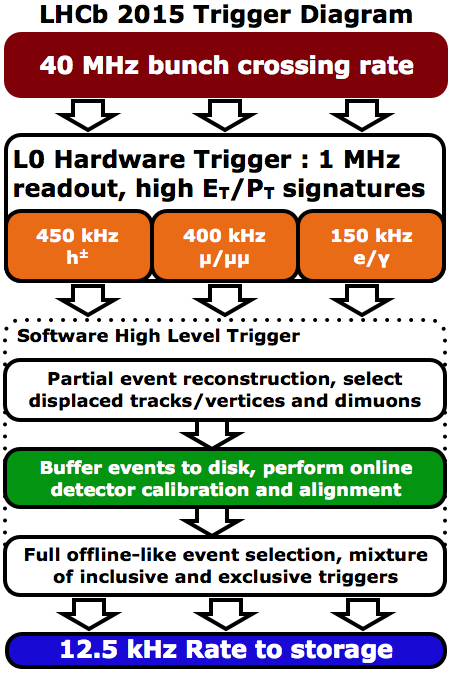
\includegraphics[width=14pc]{../figures/trigger.png}\hspace{2pc}%
\begin{minipage}[b]{14pc}\caption{\label{fig:trigger}Trigger strategy for Run~II: after the hardware stage and a first software stage based on a partial
    reconstruction, the selected events are buffered on disk while the
    real-time calibration and alignment are performed. The second
    stage of the software trigger performs the same reconstruction
    performed offline using the same calibration and alignment.}
\end{minipage}
\end{figure}

%In Run~II this deferral strategy is exploited even further as shown in Figure
%\ref{fig:trigger}; after L0 and \hltone all the selected events are buffered on
%disk allowing to have more time to process a single event (150 ms/event in
%Run~I, 350 ms/event in Run~II).  The automatic calibration and alignment is
%performed in the trigger farm within a few minutes.  The same offline
%reconstruction is run in \hlttwo thanks to this larger time budget together with
%the reduced time requested by the improved track reconstruction.


% In Run~II the LHCb trigger strategy is different as shown in Figure \ref{fig:trigger}.
% After the hardware stage, and a first software stage (\hltone) based on a partial
% reconstruction, the selected events are buffered on disk while the
% automatic calibration and alignment is performed in a few
% minutes in the trigger farm.
% The second stage of the
% software trigger (\hlttwo) performs the same reconstruction run
% offline by using the same calibration and alignment.

The \hlt is divided into two stages, \hltone and \hlttwo, processed on
an Event Filter Farm (EFF) of approximately 1700 nodes with 27000
physical cores,   which allows to simultaneosuly run 50000 processes
using hyper-threading technology.  Events selected by an \hltone
trigger are buffered to the local harddisk of each node before being
processed by \hlttwo.  This buffering is done for two purposes :
events can be processed during inter-fill periods, and the detector
can be calibrated and aligned run-by-run before the \hlttwo stage.
During 2012 LHC spent only approximately $30\%$ of its time in stable
running due to e.g.  planned technical stops, machine developement
phases and the time between data taking fills needed for the ramping
of the LHC dipole magnets.  The usage of the local disks, around
5~PBytes in total, allows around 150~hours of LHC datataking to be
buffered, and has enabled \lhcb to fully utilize the EFF throughout
the tecnical stops and machine development phases (with the exception
of the annual winter shutdown of the LHC), more than doubling the
effective available processing power.  It is this buffering which
allows the full offline event reconstruction to be executed in the
\hlttwo stage.

The \hltone trigger performs an inclusive selection of  events based
on one or two track combinations, the presence of muon tracks
displaced from the primary vertex, or dimuon combinations in the
event. Crucially, it is also able to select the types of events
required by each alignment and calibration task, and these events are
flagged by specific routing bits which allow them to be streamed to
the relevant tasks. There are two kinds of alignment and calibration
tasks : those which are expected to change for each run, and those
which are expected to change less frequently, perhaps once per fill or
once every few fills. In the first case, which mainly concerns the
calibration of the RICH detectors, the calibration constants are
calculated for each run and updated before the \hlttwo processing of
that run. In the second case, the alignment and calibration constants
are calculated for each run, and an automated monitoring task checks
if they have changed by more than a certain threshold with respect to
the previous values. When such a significant variation is observed, a
change of run is triggered. The new constants are updated for the new
run to be used online by the two stages of the software trigger, and
offline, for every further reconstruction and selection. As these
variations are infrequent and slow, the events collected in the run
preceeding this update are still reconstructed in \hlttwo and offline
with the same constants used by \hltone.  Once the detector is fully
aligned and calibrated the events are processed by \hlttwo, where a
full event reconstruction is performed. 

%As exception the RICH calibration
%constants are updated for each run after \hltone both online, in \hlttwo, and offline
%as the previous trigger stages do not rely on hadron identification
%requirements.

% This part should be moved to the introduction
This strategy has several advantages: firstly it minimises the
difference between the online and offline performance, allowing a more
effective trigger selection that can take advantage of the hadron
identification information. For example charm physics is limited by
trigger output rate contraints; using hadron identification in the
trigger allows to have a higher selection efficiency and purity for
the doubly Cabibbo suppressed modes and, at the same time, satisfy the
output rate constraints by pre-scaling the more abundant Cabibbo
favourite modes.  Secondly it ensures the stability of the alignment
quality and hence of the physics performance.  Finally, as in Run~II
the last level of the trigger performs the same reconstruction as the
one performed offline,
% \cite{Barbara}
it will be possible to run some physics analyses, with the same
offline performance, directly on the output of the trigger using the
special stream of data known as Turbo stream \cite{Sean}. This
approach has the advantage that, for some events, it will be possible
to save only the information on the signal candidate tracks ($\sim$ 5
kB per event) instead of all the electronic signals recorded from the
detector ($\sim$ 70 kB per event). This decrease of more than one
order of magnitude of the event size will allow a higher selection
rate, for example in the charm analyses that during Run~I used trigger
lines which were pre-scaled due to output rate requirements. It is
obvious that the real-time alignment and calibration becomes essential
when the raw event is not saved.



\section{The Physics Impact of Alignment and Calibration}
\textcolor{red}{Importance of alignment and of rich pid selection (example run1).
To be included also effect of alignment on ip resolution.
To be added also something about the calorimeter calibration.}

The spatial alignment of a detector and the accurate calibration of its
subcomponents are essential to achieve the best physics
performance. The correct alignment of the VELO is needed to identify primary
vertices and secondary vertices from the decay of particles containing $b$ or
$c$ quarks while a misalignment of the tracking system would degrade the
momentum and mass resolution.  Figure~\ref{fig:Upsilon} shows how an improved
alignment greatly enhances the $\Upsilon$ mass resolution from $92$ MeV$/c^2$
with the first alignment to $49$ MeV$/c^2$ with the improved one.

\begin{figure}[h]
\begin{minipage}{0.5\columnwidth}
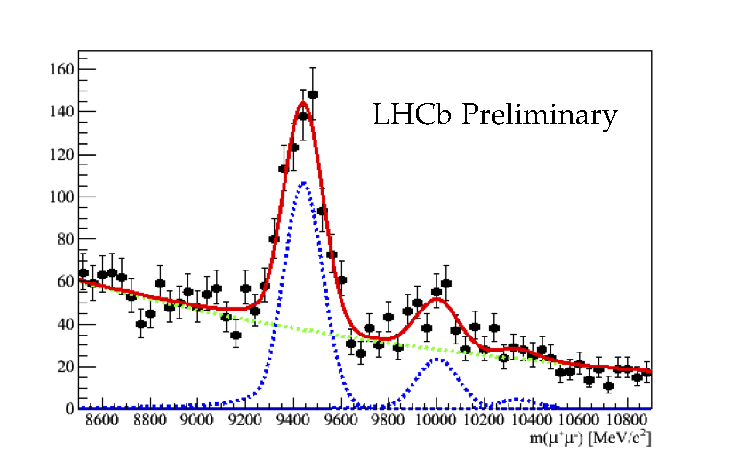
\includegraphics[width=\columnwidth]{../figures/Upsilon1}
\end{minipage}\hspace{2pc
}%
\begin{minipage}{0.5\columnwidth}
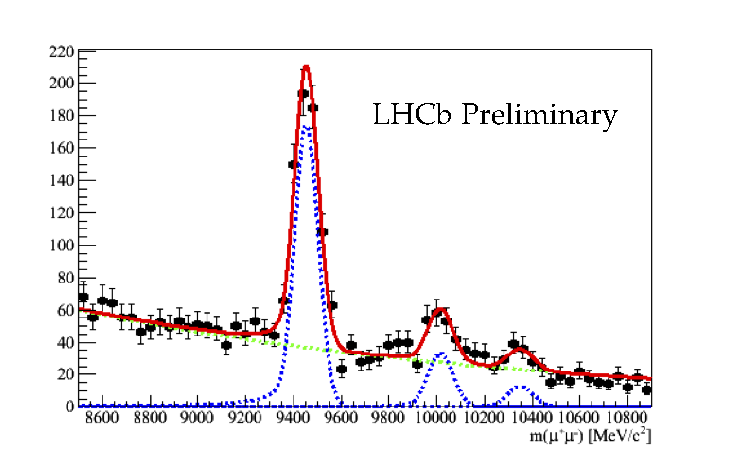
\includegraphics[width=\columnwidth]{../figures/Upsilon2}
\end{minipage} 
\caption{\label{fig:Upsilon} Invariant mass distribution for $\Upsilon \to \mu
  \mu$. The mass resolution is $92$
  MeV$/c^2$ with the first alignment (left) and is enhanced to $49$
  MeV$/c^2$ with an improved alignment (right).}
\end{figure}

An exclusive selection using hadron identification criteria relies on the
complete calibration of the ring-imaging Cherenkov
detectors. Figure~\ref{fig:PID} shows the effect in the $B^0\to h^+ h^-$ mass
spectrum of hadron identification criteria: the ratio between the signal,
$B^0\to\pi^+\pi^-$, and the combinatorial background increases by approximately
a factor two and the ratio between the signal and the favoured $B^0\to K \pi$,
increases by a factor 35.
\begin{figure}[h]
\begin{minipage}{0.5\columnwidth}
\includegraphics[width=\columnwidth]{../figures/PID1}
\end{minipage}\hspace{2pc}%
\begin{minipage}{0.5\columnwidth}
\includegraphics[width=\columnwidth]{../figures/PID2}
\end{minipage} 
\caption{\label{fig:PID} Invariant mass distribution for $B^0\to h^+ h^-$ decays~\cite{LHCb-PAPER-2012-002} in
  the LHCb data before the use of the RICH information (left), and after
  applying RICH particle identification (right). The signal under study is the
  decay $B^0\to\pi^+\pi^-$, represented by the turquoise dotted line. The
  contributions from different $b$-hadron decay modes ($B^0\to K\pi$ red dashed-dotted
  line, $B^0\to 3$-bodies orange dashed-dashed line, $B_s\to
    KK$ yellow line, $B_s\to K\pi$
  brown line, $\Lambda_b\to p K$ purple line, $\Lambda_b\to p \pi$ green line), are eliminated by
  positive identification of pions, kaons and protons. Only the signal and
  two background contributions remain visible after applying hadron
  identification requirements. The
  grey solid line is the combinatorial background.}
\end{figure}

\begin{figure}[h]
\begin{minipage}{0.5\columnwidth}
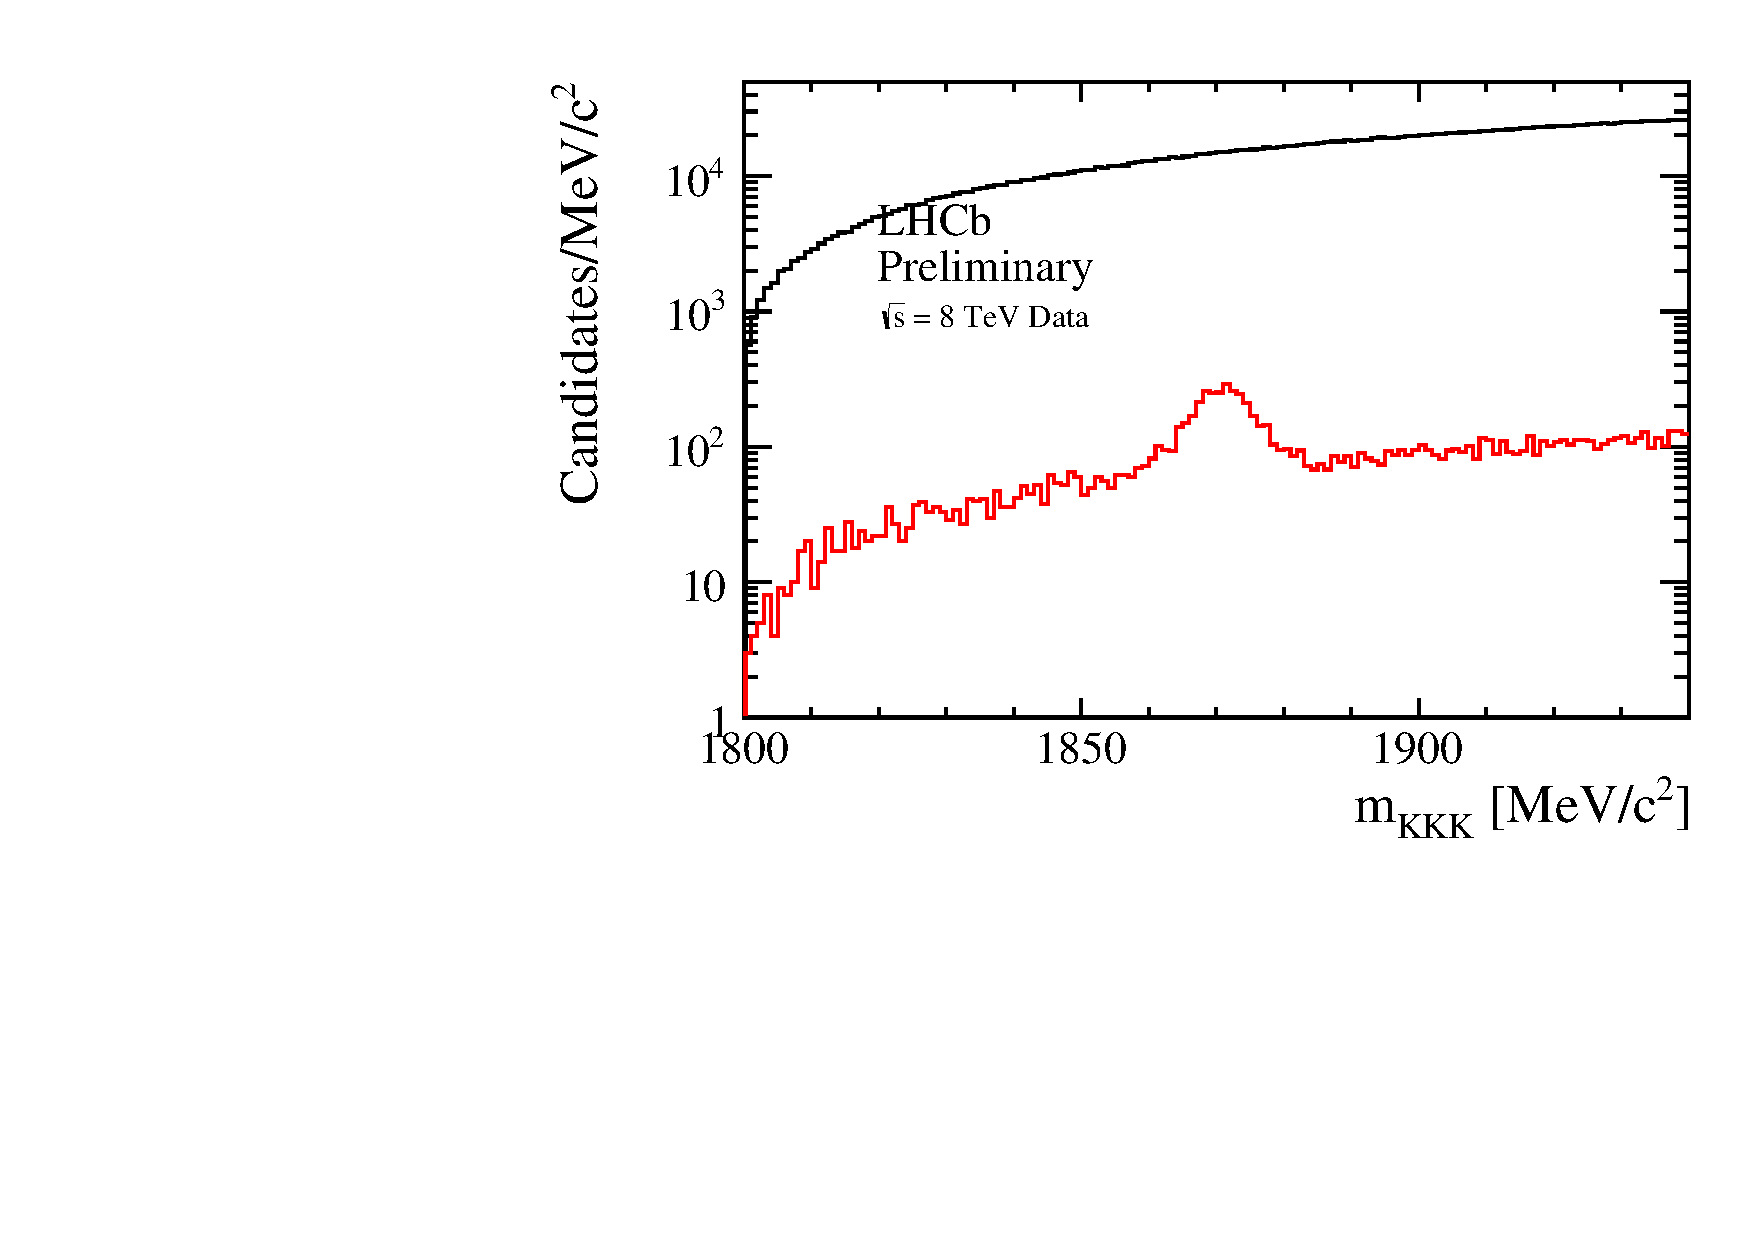
\includegraphics[width=\columnwidth]{../figures/kkk_PIDK_trigger_log}
\end{minipage}\hspace{2pc}%
\begin{minipage}{0.5\columnwidth}
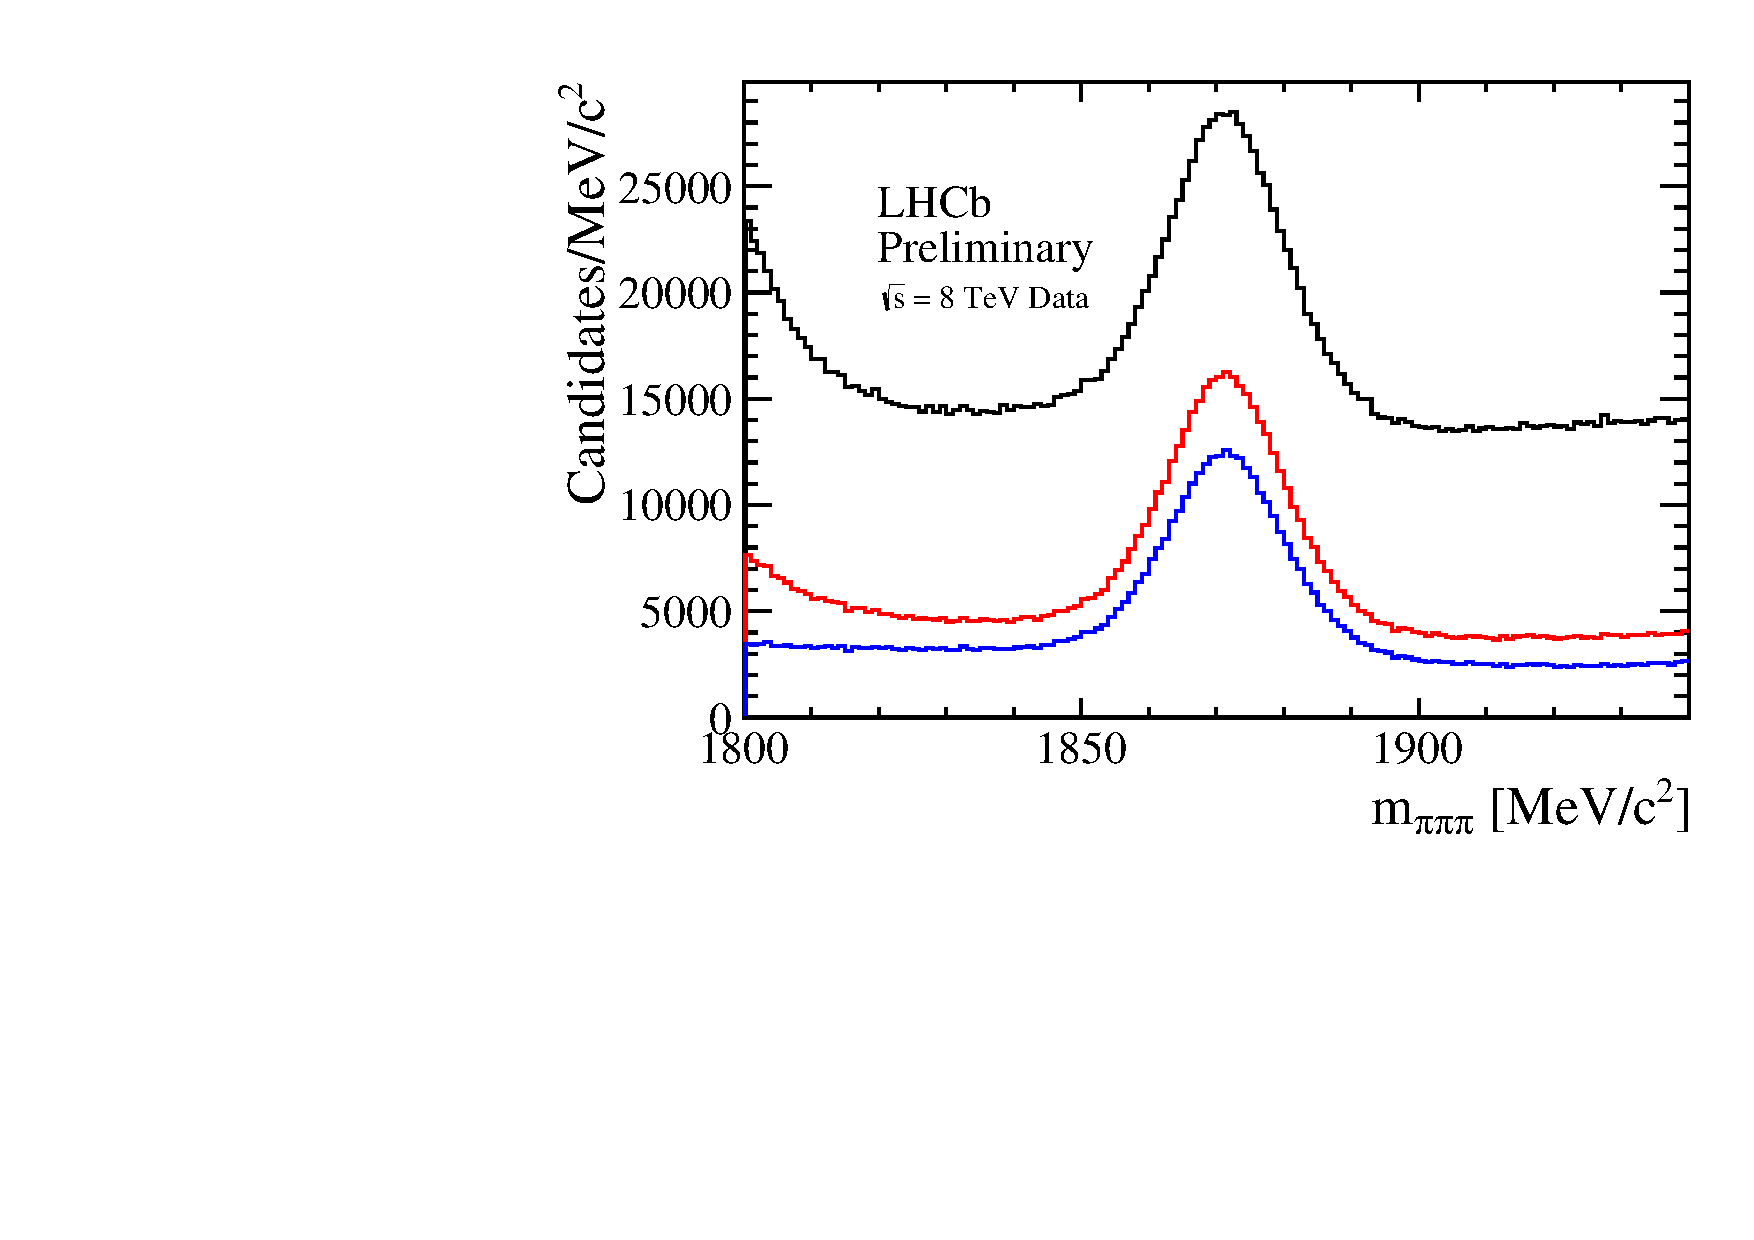
\includegraphics[width=\columnwidth]{../figures/ppp_PIDK_trigger}
\end{minipage} 
\caption{\label{fig:CharmPID} 3 body decay distribution for D0 to  kkkk (left) and pipipi (right). To be written  }
\end{figure}

Is it thus clear that using a real-time alignment and calibration during the
trigger selection allows a higher signal purity and a more effective selection
on the channels interesting to pursue LHCb's physics program without increasing
the overall trigger rate. This, however, requires us
to align more than 1700 detector components and compute almost 2000
calibration constants in real-time. It is therefore important to understand the frequency
with which the relevant constants are expected to vary.

The VELO is made of two halves that during the data taking are at approximately
8 mm away from the nominal beam position. For the safety of the detector during
the beam injection at the beginning of a fill the halves are retracted by 29 mm;
when stable beam is declared the VELO is closed around the beam.
The VELO halves are moved using stepper motors and their position is read from
resolvers mounted on the motor axes with an accuracy better than 10 $\mu$m.  An
automated closing procedure positions the VELO halves around the beams using the
response of the hardware and the measured positions of the beams.  By
considering the two independent beam profiles compiled by each half, the VELO is
observed to close symmetrically around the beams to an accuracy of better than 4
$\mu$m.  As the VELO is closed for each fill, its alignment may change with the
same frequency.

Figure \ref{fig:alignStability} shows for a subsample of the Run~I dataset the
variation of the misalignment between the two halves in the horizontal direction
perpendicular to the beam. It can be estimated by taking the difference of the
positions of the primary vertices reconstructed separately with tracks in only
one half of the VELO. In a perfectly aligned detector the mean of this
difference should be zero. The average variation in Run~I is $\sim 4\,\mu$m
while the maximum variation is $O(10\,\mu$m$)$, which is more than the
$O(2\,\mu$m$)$ precision of the track based software alignment procedure
\cite{LHCb-DP-2014-001}.

\begin{figure}[h]
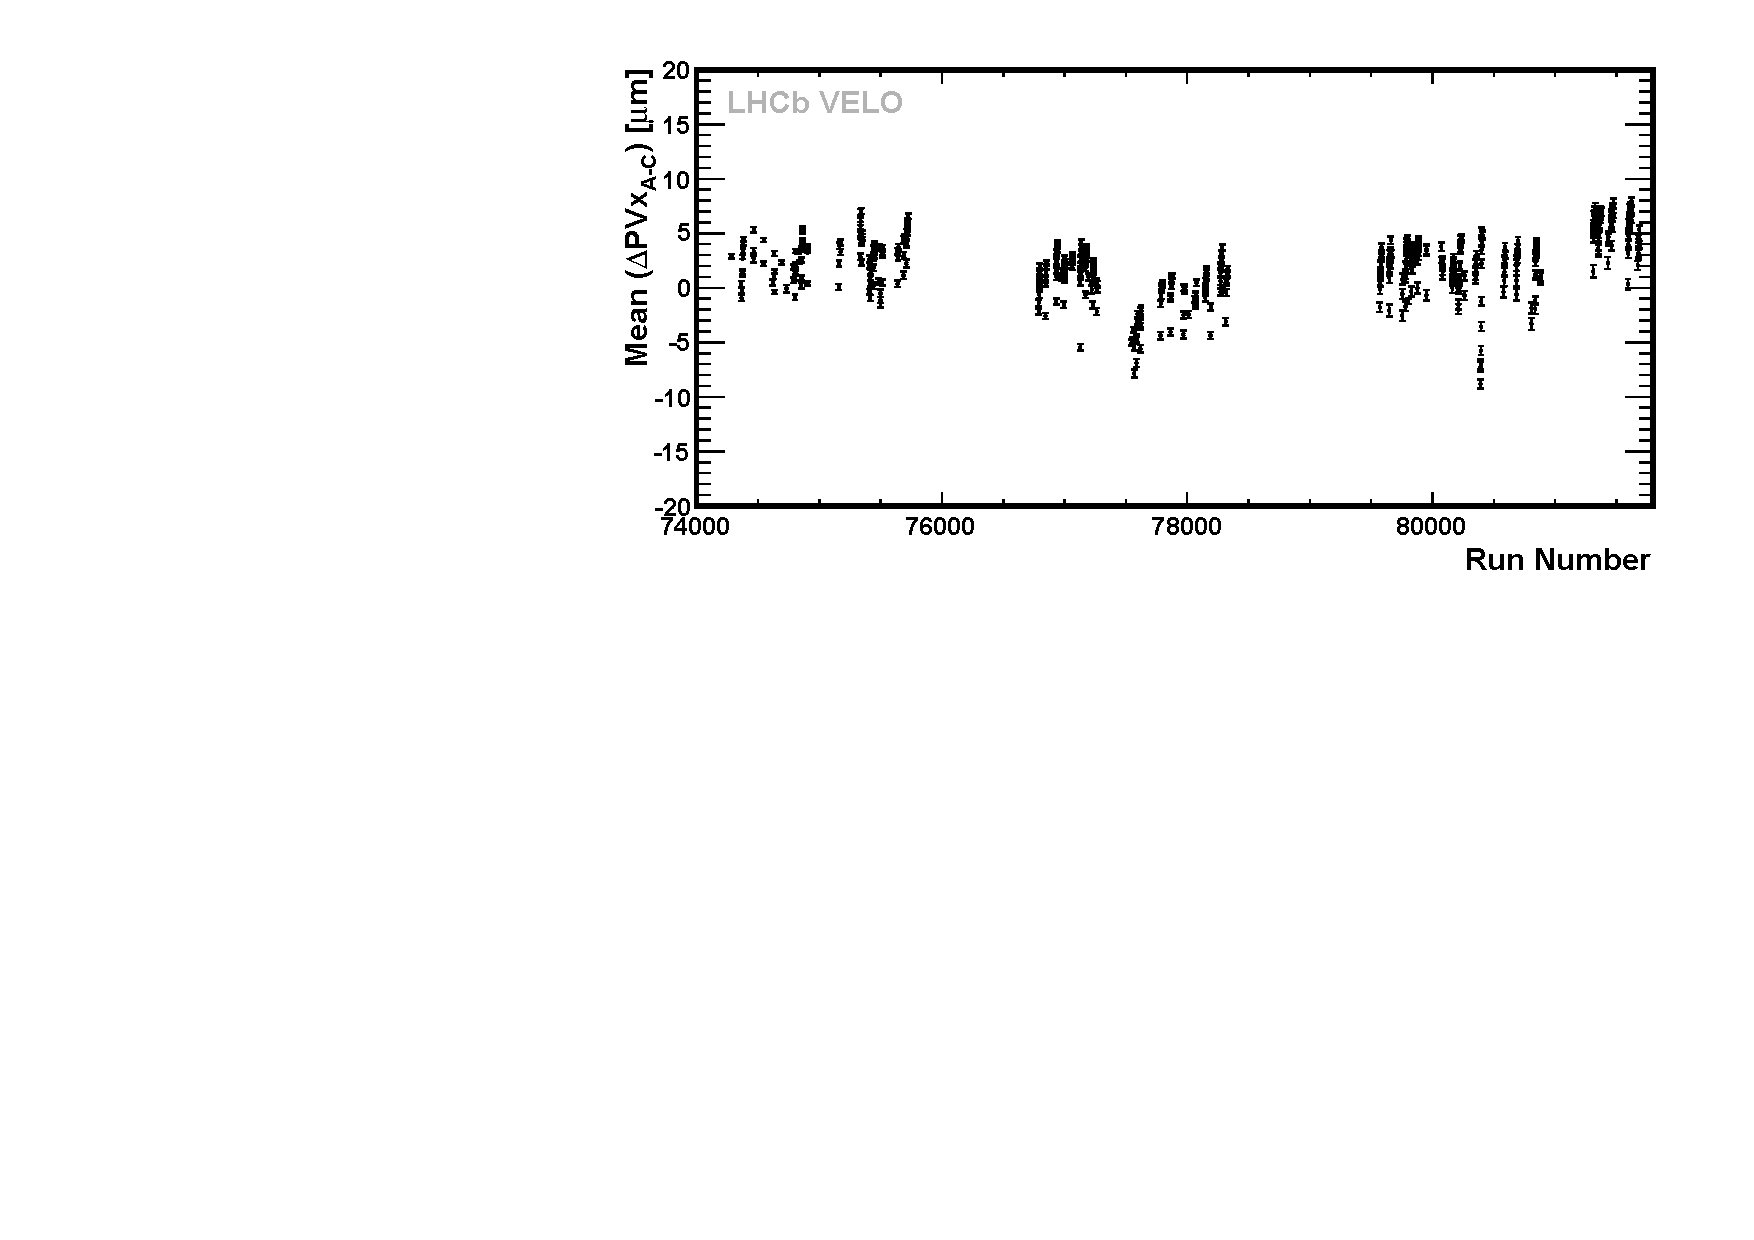
\includegraphics[width=20pc]{../figures/alignStability}\hspace{2pc}%
\begin{minipage}[b]{14pc}\caption{\label{fig:alignStability}
    Misalignment 
    between the two VELO halves along the main movement direction
    for the different runs, evaluated by fitting the primary
    vertices separately with tracks in each half of the VELO. 
The run numbers shown here span the period of the last four months of operations in 2010.}
\end{minipage}
\end{figure}

For the other components of the tracking system, in addition to the variation
due to hardware intervention, some variation over time was observed, partially
correlated to the magnet polarity which is reversed periodically. During Run~I a
new tracking alignment has been evaluated after each magnet polarity switch or
technical stop.  This strategy allowed to have a momentum scale and resolution
stable with time as shown in Figure \ref{fig:trackerStability}.

\begin{figure}[h]
\begin{minipage}{0.5\columnwidth}
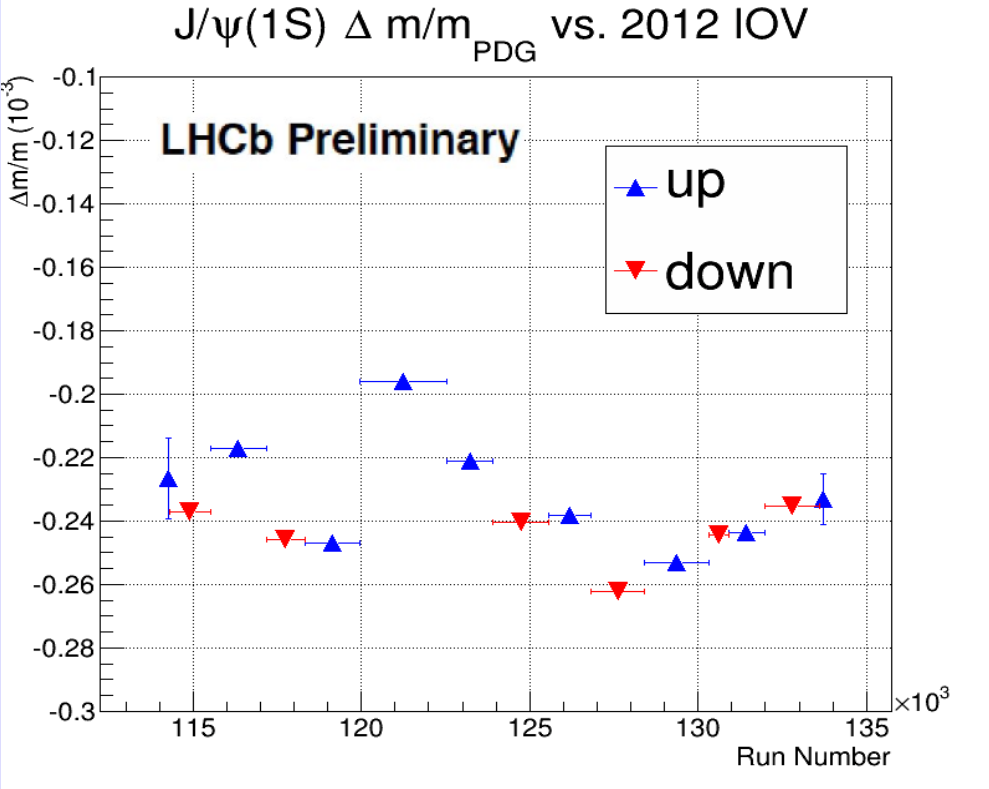
\includegraphics[width=\columnwidth]{../figures/JPsi1.png}
\end{minipage}\hspace{2pc}%
\begin{minipage}{0.5\columnwidth}
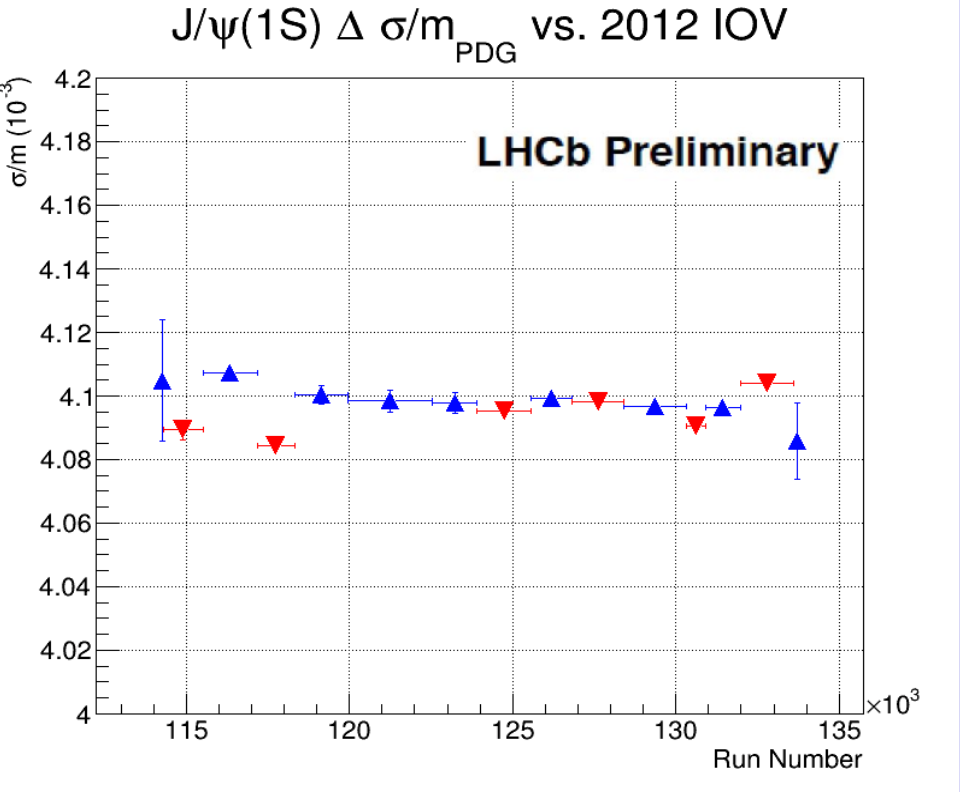
\includegraphics[width=\columnwidth]{../figures/JPsi2.png}
\end{minipage} 
\caption{\label{fig:trackerStability} Time evolution of  the relative variation of the difference
  between the measured mass of the $J/\Psi$(1S) and the nominal one from
  \cite{PDG} (left) and relative variation of the mass resolution at the
  $J/\Psi$(1S) mass (right). Each point corresponds to data taken with a
  different tracking alignment; the blue up-triangles and red down-triangles correspond to opposite magnet polarities.}
\end{figure}

Finally, in the case of the gaseous RICH detectors, the variations of temperature
and pressure in the experimental cavern mean that the refractive index of the gas
changes continuously. In order to achieve the best particle identification performance, it 
is necessary to compute these constants for each run. On the other hand, the alignment
of the RICH mirrors is seen to vary only infrequently, and in general only needs to be updated
after an extended shutdown of the detector. \textbf{DO WE HAVE SOME JUSTIFICATION?}

\textbf{SAY SOMETHING ABOUT THE EXPECTED VARIATION OF THE CALO HERE?}



\section{The Online Alignment Framework}

To allow the calibration and alignment tasks to operate, they have been embedded
in the online system in terms of data flow and control flow.

\subsection{Data Flow}

All of the tasks make use of events that have been accepted by the HLT1 stage of
the High Level Trigger. The alignment tasks require events with specific
content such as decays of \decay{\Dz}{\kaon\pion} or \decay{\jpsi}{\mup\mum}, or
tracks with specific properties. The calibration tasks have no requirements on
the event content, but do require a sufficient number of events to fill the
distributions used to obtain the calibration constants.

Events for the alignment tasks are selected by dedicated selections that are
part of HLT1 and, based on acceptance by these selections, written to files on
the hard-drives installed in the farm nodes. The number of events written to
files across the farm is tracked and once a sufficient number for a given task
has been accumulated, the tasks writing events are stopped, until a new sample
is required. The Velo alignment requires 

Approximately a kilohertz of events accepted by HLT1 is transferred over the
network to dedicated tasks that processes as many of these events as they
can. These tasks provide the distributions required to perform the calibration,
and write them to files. The files are written every fifteen minutes and at
least once per run, which is a period of data-collection up to an hour long.

\subsection{Control Flow}

\begin{figure}[h]
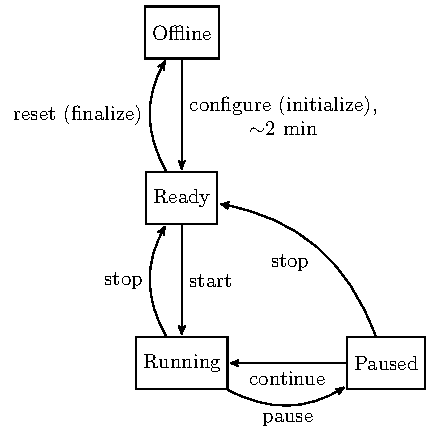
\includegraphics[width=5cm]{../figures/FSM}
\caption{Finite state machine that defines the behaviour of the alignment
  tasks.}
\label{fig:FSM}
\end{figure}

The Outer Tracker calibration and RICH refractive index calibration tasks run
independently from ECS and wait for the files containing the distributions they
require. Once a file becomes available for a given run, the calibration
algorithms are triggered to process the distributions, and if a new set of
calibration constants is created, write these to a file. The ECS is then
informed of the availability of the new versions and which run(s) these
correspond to.

The execution of the alignment tasks is under the control of the LHCb Experiment
Control System (ECS), and is implemented as a finite state machine, which is
shown in \cref{fig:FSM}. Once FSM reaches the initial ``READY'' state, it will
loop from ``READY''$\to$``RUNNING''$\to$``PAUSED''$\to$``READY'' until it stops
when a convergence criterium is satisfied.

The task that steers the iterations is called the iterator and the tasks that
analyze the data are called the analyzers; both tasks follow the same sequence
of states. When all tasks are in the ``READY'' state, the iterator makes an
initial set of alignment constants available to the analyzers and then updates
its state to ``RUNNING''. The analyzers are then sent the ``start'' command,
update their state to ``RUNNING'' and start analyzing their data. Each analyzer
that has completed processing its data updates its state to ``PAUSED'', and once
they have all reached this state, they are sent the ``stop'' command and update
their state to ``READY''. The iterator is then sent the ``pause'' command,
collects and combines the output produced by the analyzer tasks and either
indicates that conversion has been reached by updating its state to ``READY'',
or that further iteration is required by producing a new set of constants and
updating its state ``RUNNING''. If the iterator decides that the process has
converged and the changes in the alignment constants are above a given
threshold, it writes the new alignment constants to a file and announces the new
version to the control system.


\section{Alignment and Calibration Tasks}


\section{Alignment and Calibration Tasks}

\subsection{Tracking Alignment}
\subsubsection{Alignment method}
\textcolor{red}{give more details}

The tracking alignment is based on an iterative procedure where the
residuals of a Kalman track fit are minimised.  The magnetic field and
material effects are taken into account and information from vertices
and particle masses can also be used as constraints to avoid global
distortions \cite{Hulsbergen,AlignConstraints}. 

Given a set of tracks reconstructed using the alignment parameters
$\alpha_0$, the new set of alignment constants can be found solving
the system of equations
\begin{equation}
\alpha = \alpha_0 -\left.\left(\frac{d^2 \chi^2}{d\alpha^2}
\right)^{-1} \right|_{\alpha_0}  \left.\frac{d
  \chi^2}{d\alpha}\right|_{\alpha_0},
\label{eq:minimize}
\end{equation}
where the derivatives of the total $\chi^2$ with respect to the
alignment parameters are obtained by summing the contributions from
all the tracks:
\begin{equation}
\begin{aligned}
\frac{d \chi^2}{d\alpha} &= 2 \sum_{\mbox{tracks}}
\frac{dr}{d\alpha}^T V^{-1} r ,\\ \frac{d^2 \chi^2}{d\alpha^2} &= 2
\sum_{\mbox{tracks}} \frac{dr}{d\alpha}^T V^{-1} R V^{-1}
\frac{dr}{d\alpha}.\\
\end{aligned}
\label{eq:derivatives}
\end{equation}
Here $V$ is the covariance matrix of the measurement coordinates, $r$
is the track residuals (the distance between the hit position and the
track intercept point), and $R$ is the covariance matrix of the
residuals. It is assumed that the $\chi^2$ has been minimised with
respect to the track parameters for the alignment $\alpha_0$.

\subsubsection{VELO Alignment}
\textcolor{red}{ it should include (random order):stability plots, variation of the constants, time needed to run the jobs, event selections. Performance before/aftera alignment. Trend of the constants and evaluation of the variation. Maybe trends of physics quantity like mass or time resolution}

\subsubsection{Tracker Alignment}

\subsubsection{Muon Alignment}


\subsection{\rich Mirror Alignment}
\textcolor{red}{This should include, description of the method (detector description
should be included in previous section), data selected, time required 
for this task, performance (before/after alignment) and stability of the constants. 
The overall performance, maybe also stability of the overall performance (PID 
or/and cherenkov angle resolution) could be together for calibration and alignment.}



Both \rich detectors have two sets of mirrors: photons are reflected off a
primary mirror onto a secondary mirror, from where they are deflected out of the
LHCb acceptance onto the photodetector plane.
\begin{figure}[h]
\begin{center}
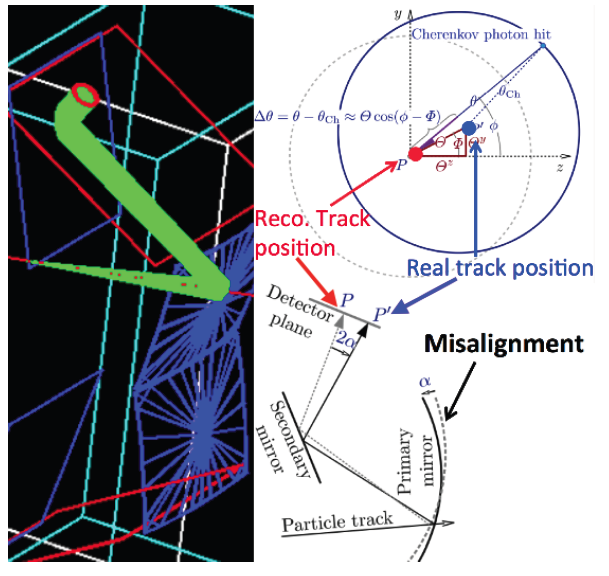
\includegraphics[width=0.7\textwidth]{../figures/RichMissAlign.png}
\caption{\label{fig:RichMissAlign} Left: 3D representation of a track (red line) going through a radiator and emitting Cherenkov photons (green cone). The photons are reflected by a spherical primary mirror (blue rectangle with star-shaped pattern) onto a flat secondary mirror (blue rectangle) and from there onto the photodetector plane (red rectangle). The observable Cherenkov ring is shown as a red circle on the photodetector plane. Right: Schematic illustration of the effects of a misalignment in the \rich mirror system. The projected track position on the photodetector plane $P$ is displaced by $\varTheta^z$ and $\varTheta^y$ with respect to the the actual center of the Cherenkov ring on the photodetector plane $P'$. The Cherenkov angle $\theta$ is evaluated relative to $P$ and varies with the azimuthal angle $\phi$.}
\end{center}
\end{figure}

Any misalignment of the \rich detectors with respect to the tracking system is observed as a shift of the track projection point on the photodetector plane from the center of its corresponding Cherenkov ring as is illustrated in Figure \ref{fig:RichMissAlign}. This shift is observed by analysing the Cherenkov angle, $\theta$, as a function of the azimuthal Cherenkov angle $\phi$, defined as the angle of the pixel hit in the coordinate system of the photodetector plane, with the projected track coordinate at the origin. For a well aligned detector the angle $\theta$ is independent of the angle $\phi$, whilst a misaligned system results in a sinusoidal distribution as shown in Figure \ref{fig:RichMirror}.\\
In practice, distributions of $\Delta \theta$ against $\phi$ are plotted for each possible combination of primary and secondary mirror, where $\Delta \theta (\phi) = \theta(\phi) - \theta_{\mathrm{Ch}}$ and $\theta_{\mathrm{Ch}}$ is the Cherenkov angle calculated from the momentum of the track and the refractive index of the radiator \cite{LHCb-DP-2012-003}. Any systematic shift away from the value $\theta_{\mathrm{Ch}}$ is observable as a shift in $\Delta \theta$. \\
The $\Delta \theta$ distribution is then divided into slices in $\phi$. For each slice, a one dimensional histogram of $\Delta \theta$ is fitted with a Gaussian plus a second order polynomial background, where the means of the Gaussians of the different slices are connected in the fit by a sinusoidal distribution given by 
\begin{equation}
\begin{aligned}
 \Delta \theta_{p,s} (\phi) & \equiv   [\theta(\phi)-\theta_{\mathrm{Ch}} ]_{p,s} \\
                            &    =         \varTheta^z_{p,s}\cos\phi
                                 +         \varTheta^y_{p,s}\sin\phi                 \\
\end{aligned}
\end{equation}
The final fit is shown in Figure \ref{fig:RichMirror}; the extracted values of $\varTheta^y_{p,s}$ and $\varTheta^z_{p,s}$ correspond to the misalignment on the  photodetector plane for a mirror combination of primary mirror $p$ and secondary mirror $s$ in the $y$ and $z$ direction respectively.\\
The alignment of the mirror segments has the extra complication that every photon is reflected twice, and thus the data must be separated into samples which have unique primary and secondary mirror combinations. For this procedure, only photons that can be uniquely associated to a given mirror combination are used. \\
%Mirror segments are identified by considering photons to have been emitted at both the start and end of the gas radiators. If the mirror segments reflecting the photons are the same in both cases, the photon trajectory is considered \textit{unambiguous} and is used for the alignment of mirror segments.\\
The mirror arrangement in \richone allows for alignment using a sequential approach, where the primary mirrors are aligned first, followed by the secondary mirrors. This is possible because photons reaching a particular secondary mirror can only be reflected from a single primary mirror. In \richtwo the larger number of primary/secondary mirror combinations makes the use of a sequential method impossible. The alignment of the \richtwo mirror segments is performed by solving a set of simultaneous equations to extract all the alignment parameters of all the mirrors. In general two iterations of this method are required to obtain the final mirror alignment.\\
\\
\begin{figure}[h]
\begin{minipage}{0.5\columnwidth}
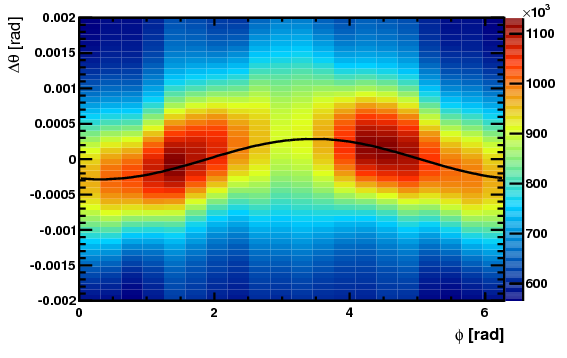
\includegraphics[width=\columnwidth]{../figures/RichMirror1.png}
\end{minipage}\hspace{2pc}%
\begin{minipage}{0.5\columnwidth}
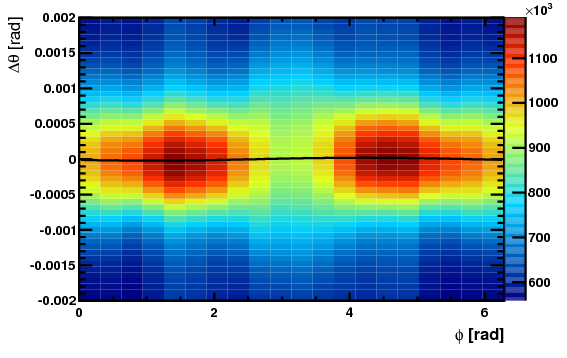
\includegraphics[width=\columnwidth]{../figures/RichMirror2.png}
\end{minipage} 
\caption{\label{fig:RichMirror} Difference between the measured and
  expected Cherenkov angle $\Delta\Theta$ as a function of the azimuthal angle $\phi$ before
  (left) and after (right) the mirror alignment for one mirror \cite{LHCb-DP-2012-003}.}
\end{figure}
As for the tracker alignment, the \richone and \richtwo alignments are performed on events collected by their respective \hltone lines. The \hltone lines for the \rich alignments trigger on high energy tracks whose Cherenkov photons would populate the outermost mirror combinations. The other mirror combinations are populated by the other tracks in the events. All tracks entering the alignment procedure have to have a momentum $p$ greater than 20(40)\gev for \richone (\richtwo) in order for the Cherenkov angle to be saturated and therefore $\theta_{\mathrm{Ch}}$ be predictable from the track momentum and the refractive index of the radiator.\\
The event reconstruction and filling of the $\Delta \theta$ vs. $\phi$ histograms is done by the analysers in parallel. The individual histograms are collected and merged and then fitted by the iterator. The iterator also determines the individual mirror misalignments and creates a new database slice with the mirror orientations and decided weather the alignment procedure has converged or if another iteration needs to be started. The alignment procedure takes about XXX for \richone and XXX for \richtwo.\\
MORE ON STABILITY AND PERFORMANCE TO COME SOON.\\
\subsection{Rich Calibration}
\textcolor{red}{This should include, description of the method (detector description
should be included in previous section), data selected, time required 
for this task, performance (before/after calibration) and stability of the constants
or variation as function of temperature/pressure. 
The overall performance, maybe also stability of the overall performance (PID 
or/and cherenkov angle resolution) could be together for calibration and alignment.}

The RICH automatic calibration consists of calibrating the RICH refractive index
and the Hybrid Photon Detectors (HPDs) images. Both these calibrations are
evaluated and updated every run.

The refractive index of the gas radiators depends on the ambient temperature and
pressure, and the exact composition of the gas mixture and so can change in
time.  These quantities are monitored to compute an expected refractive index,
but this does not have a high enough precision and needs to be corrected.  The
distribution of the difference between the reconstructed and expected Cherenkov
angle is fitted to extract the scale factor to correct the expected refractive
index.

\begin{figure}[h]
  \centering
  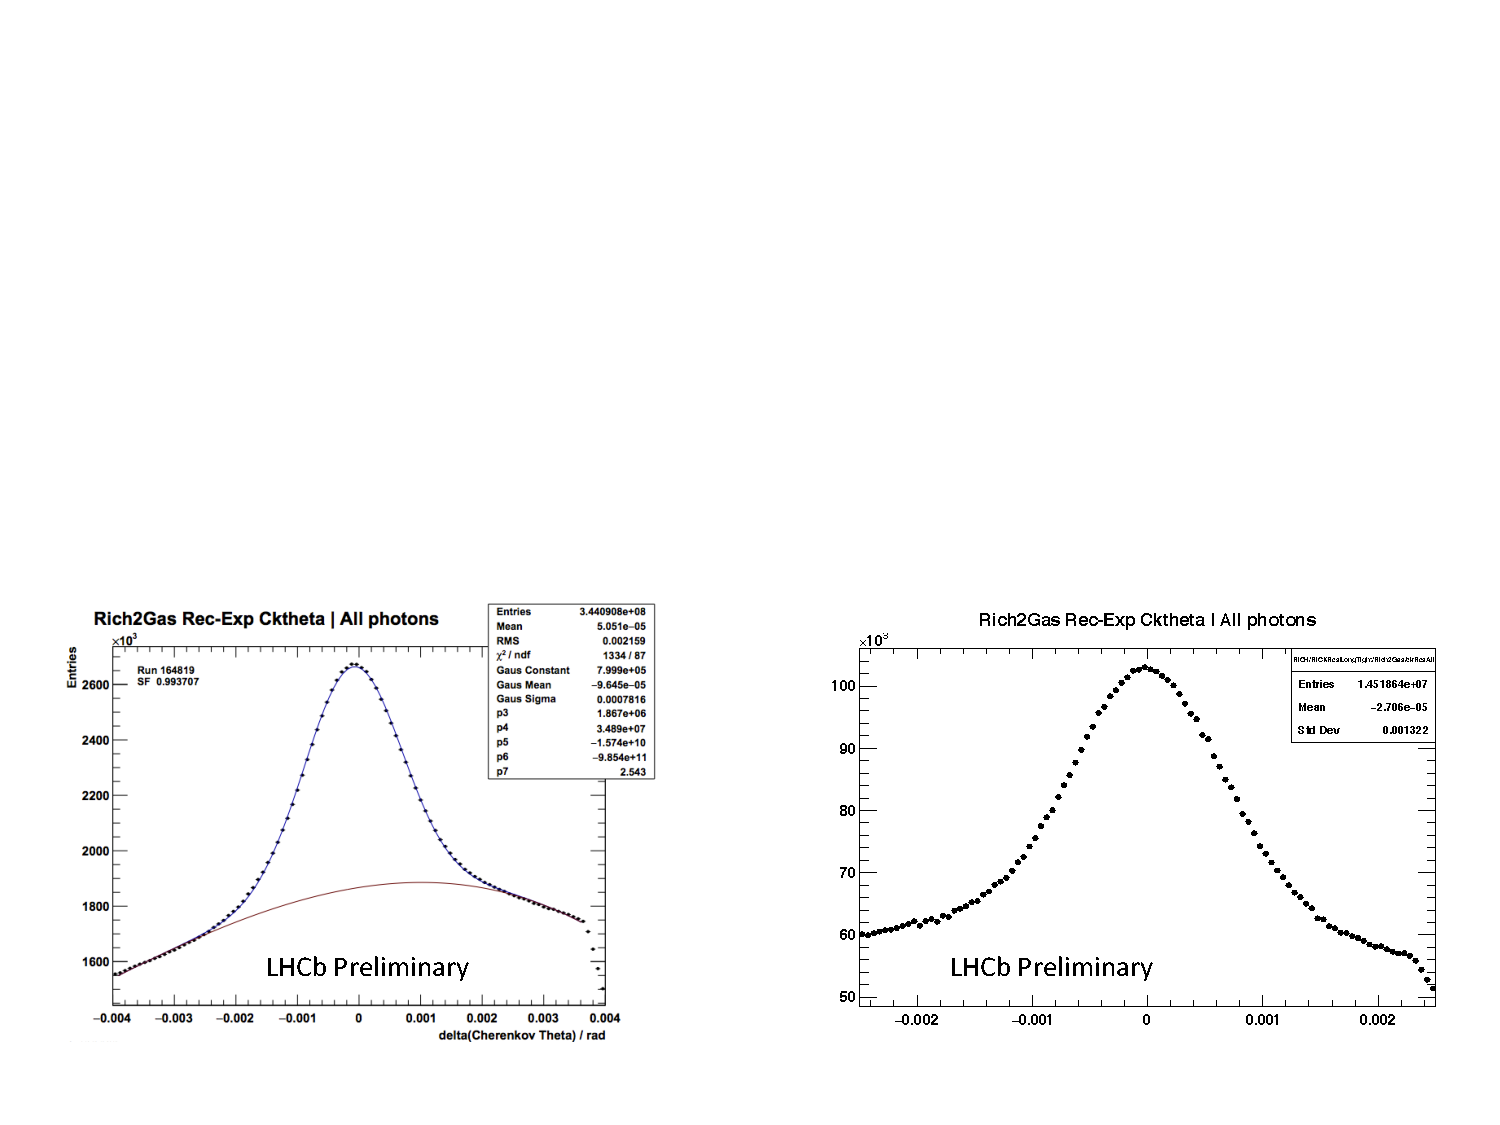
\includegraphics[width=8cm]{../figures/RichCalibration}
\caption{RICH cherenkov angle before (left) and after (right) the calibration,Caption to be written, 1st draft for the plot}
  \label{fig:RichCal}
\end{figure}

%due righe per spiegare HPD
HPDs are used to detect Cherenkov photons. They consist of vacuum tubes
separated from the radiator gas by a quartz window and a photocathode. The
photoelectrons produced are focused onto a silicon pixel array using an
accelerating voltage \cite{LHCb-DP-2012-003}.  The anode images are affected by
magnetic and electric fields, and so are cleaned and a Sobel filter \cite{Sobel}
is used to detect the edges. Figure \ref{fig:RichCal} shows the anode images
before and after this process. The evaluation of the new calibration constants
does not require an iterative procedure and can be obtained by fitting the
relevant distribution on a single node.

\begin{figure}[h]
  \centering
  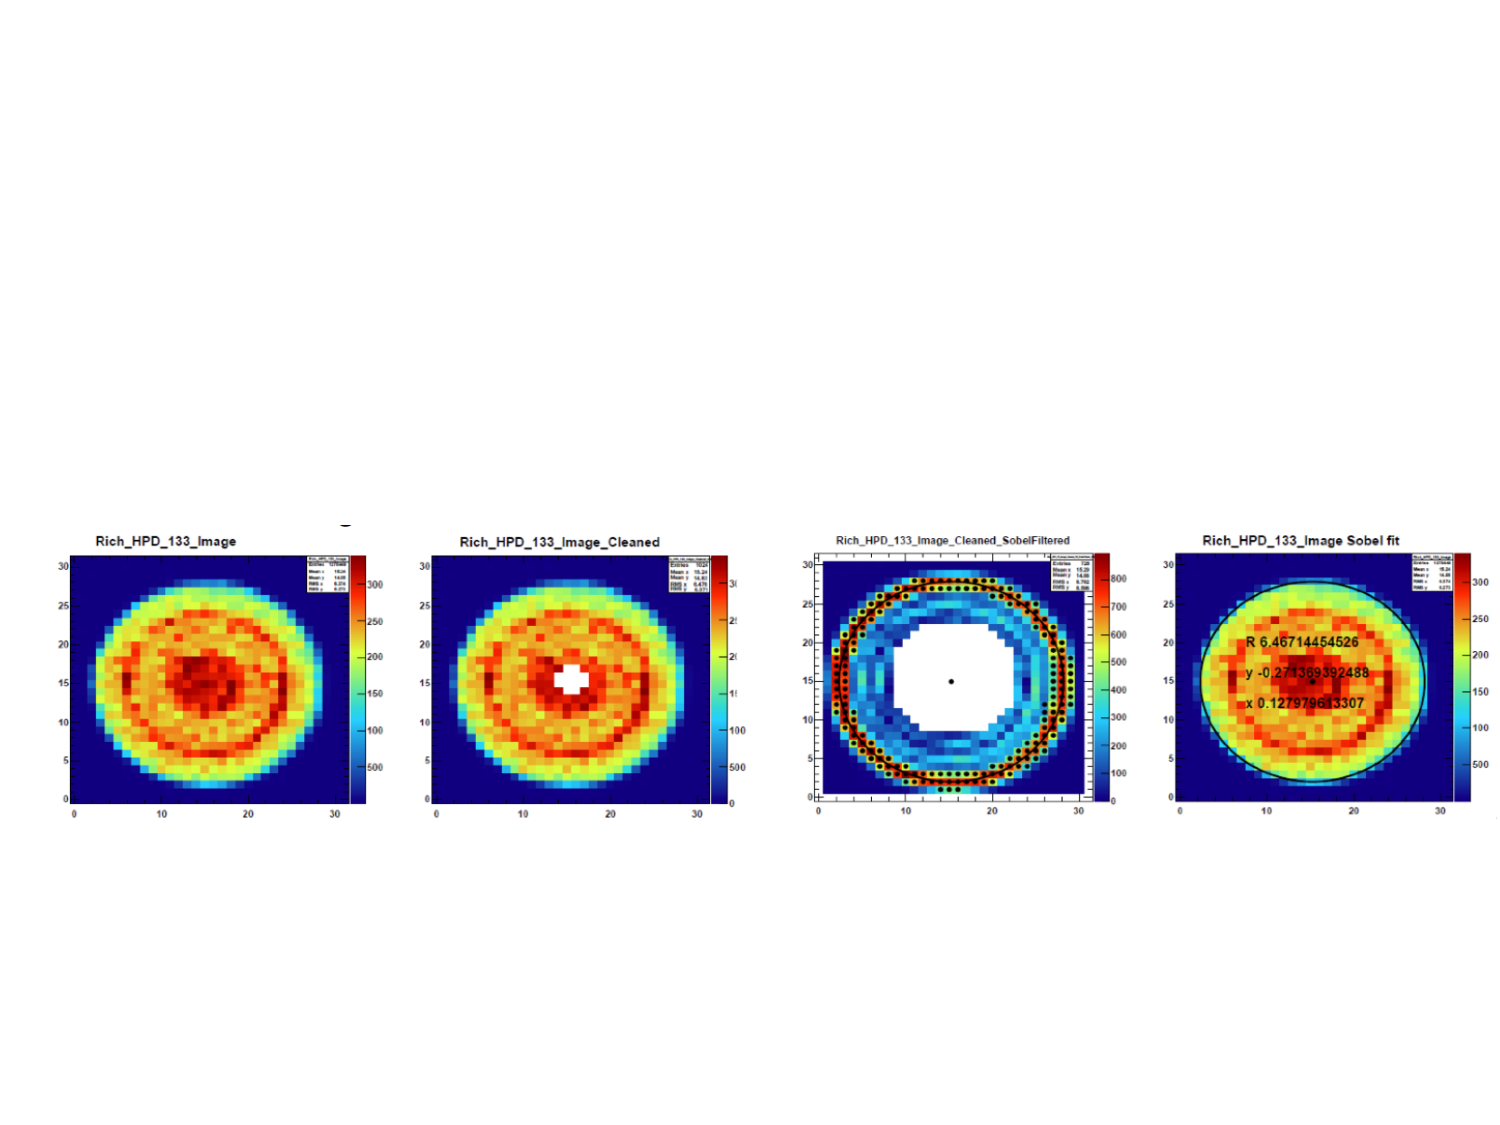
\includegraphics[width=8cm]{../figures/RichHPDCalibration}
\caption{RICH HPD anode images,Caption to be written, 1st draft for the plot.
%before (left) and after(right) the cleaning and applying the Sobel filter.
}
  \label{fig:RichHPDCal}
\end{figure}



\subsection{OT Calibration}

\begin{figure}[h]
  \centering
  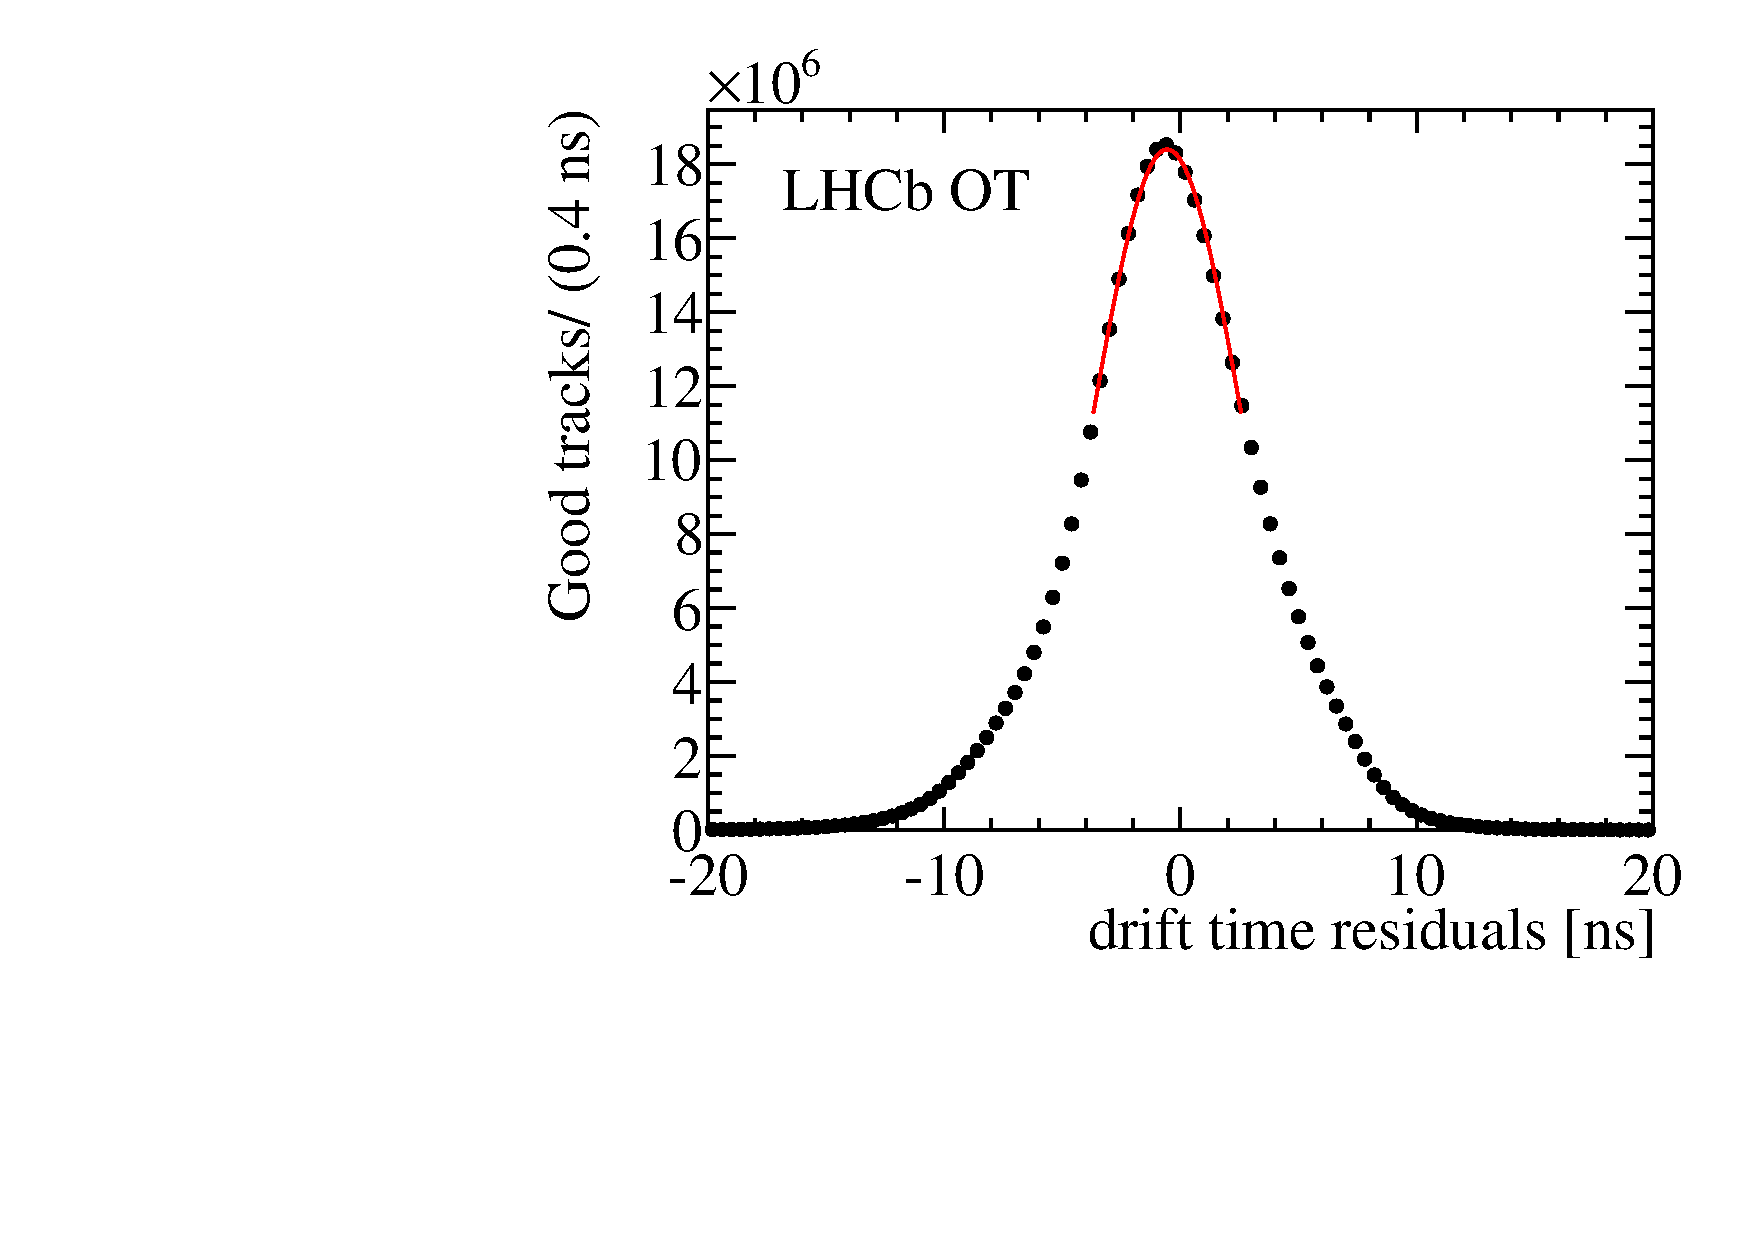
\includegraphics[width=8cm]{../figures/OT_fit}
  \caption{Fit to the distribution of the drift-time residuals of Outer Tracker
    hits, used to estimate the global time offset between the collision time and
    the LHC clock.}
  \label{fig:OT_calib}
\end{figure}

The LHCb Outer Tracker (OT) \cite{LHCb-DP-2013-003} is a detector consisting of
gas-filled straws with a 5 mm pitch. The time difference between a bunch
crossing and the measurement of a signal in one of the straws,
$t_{\text{meas}}$, consists of several compenents as expressed by:
\begin{equation}
  t_{\text{meas}} = t_0 + t_{\text{flight}} + t_{\text{prop}} + t_{\text{drift}},
\end{equation}
where $t_0$ is the time delay caused by the readout electronics,
$t_{\text{flight}}$ is the time-of-flight of the charged particle that caused
the signal, $t_{\text{prop}}$ is the time required for the signal to propagate
along the wire to the readout electronics, and $t_{\text{drift}}$ the drift-time
of electrons in the gas.

While the $t_0$ time delay is different for each read-out board of the OT, it
can be written as the sum of a average, detector-wide, offset and a per-board
offset. As the per-board offsets are a property of the electronics, they are
expected to change very little. The global offset changes more frequently as a
result of, for example, drift of the arrival time of the LHC clock to which the
readout is synchronised. To correct for these global clock changes, a
near-realtime analysis is performed to calibrate it.

Data accepted by the HLT1 stage of the HLT is sent to a small farm running of
$O(50)$ of the LHCb reconstruction application, Brunel. Good quality tracks
that traverse the Velo and OT are selected and the expected drift-times of hits
in the OT are calculated from the track parameters. The residual differences
between the expected and measured drift-times are entered into a histogram and a
fit of a Gaussian function to the central part of the resulting distribution is
performed to extract the global offset. An example of such a fit it shown in
\cref{fig:OT_calib}.

Data is collected in LHCb in periods of up to an hour long, called runs. The
calibration is performed at most once per run once a distribution of drift-time
residuals of sufficient size has been obtained; fifty thousand entries are
typically sufficient. The task that performs the calibration waits for the
distribution of drift-time residuals to be made available to it, which occurs
approximately every fifteen minutes, and at the end of a run. The calibration is
then performed and if the difference with the last known best calibration is
larger than a threshold, the new calibration is saved and automatically
propagated to all tasks running online at the start of the next run; it is also
inserted into the database used by tasks running
offline. \Cref{fig:OT_calib_time} shows the values of the global time offset
obtained during July and August of 2015.

\begin{figure}[h]
  \centering
  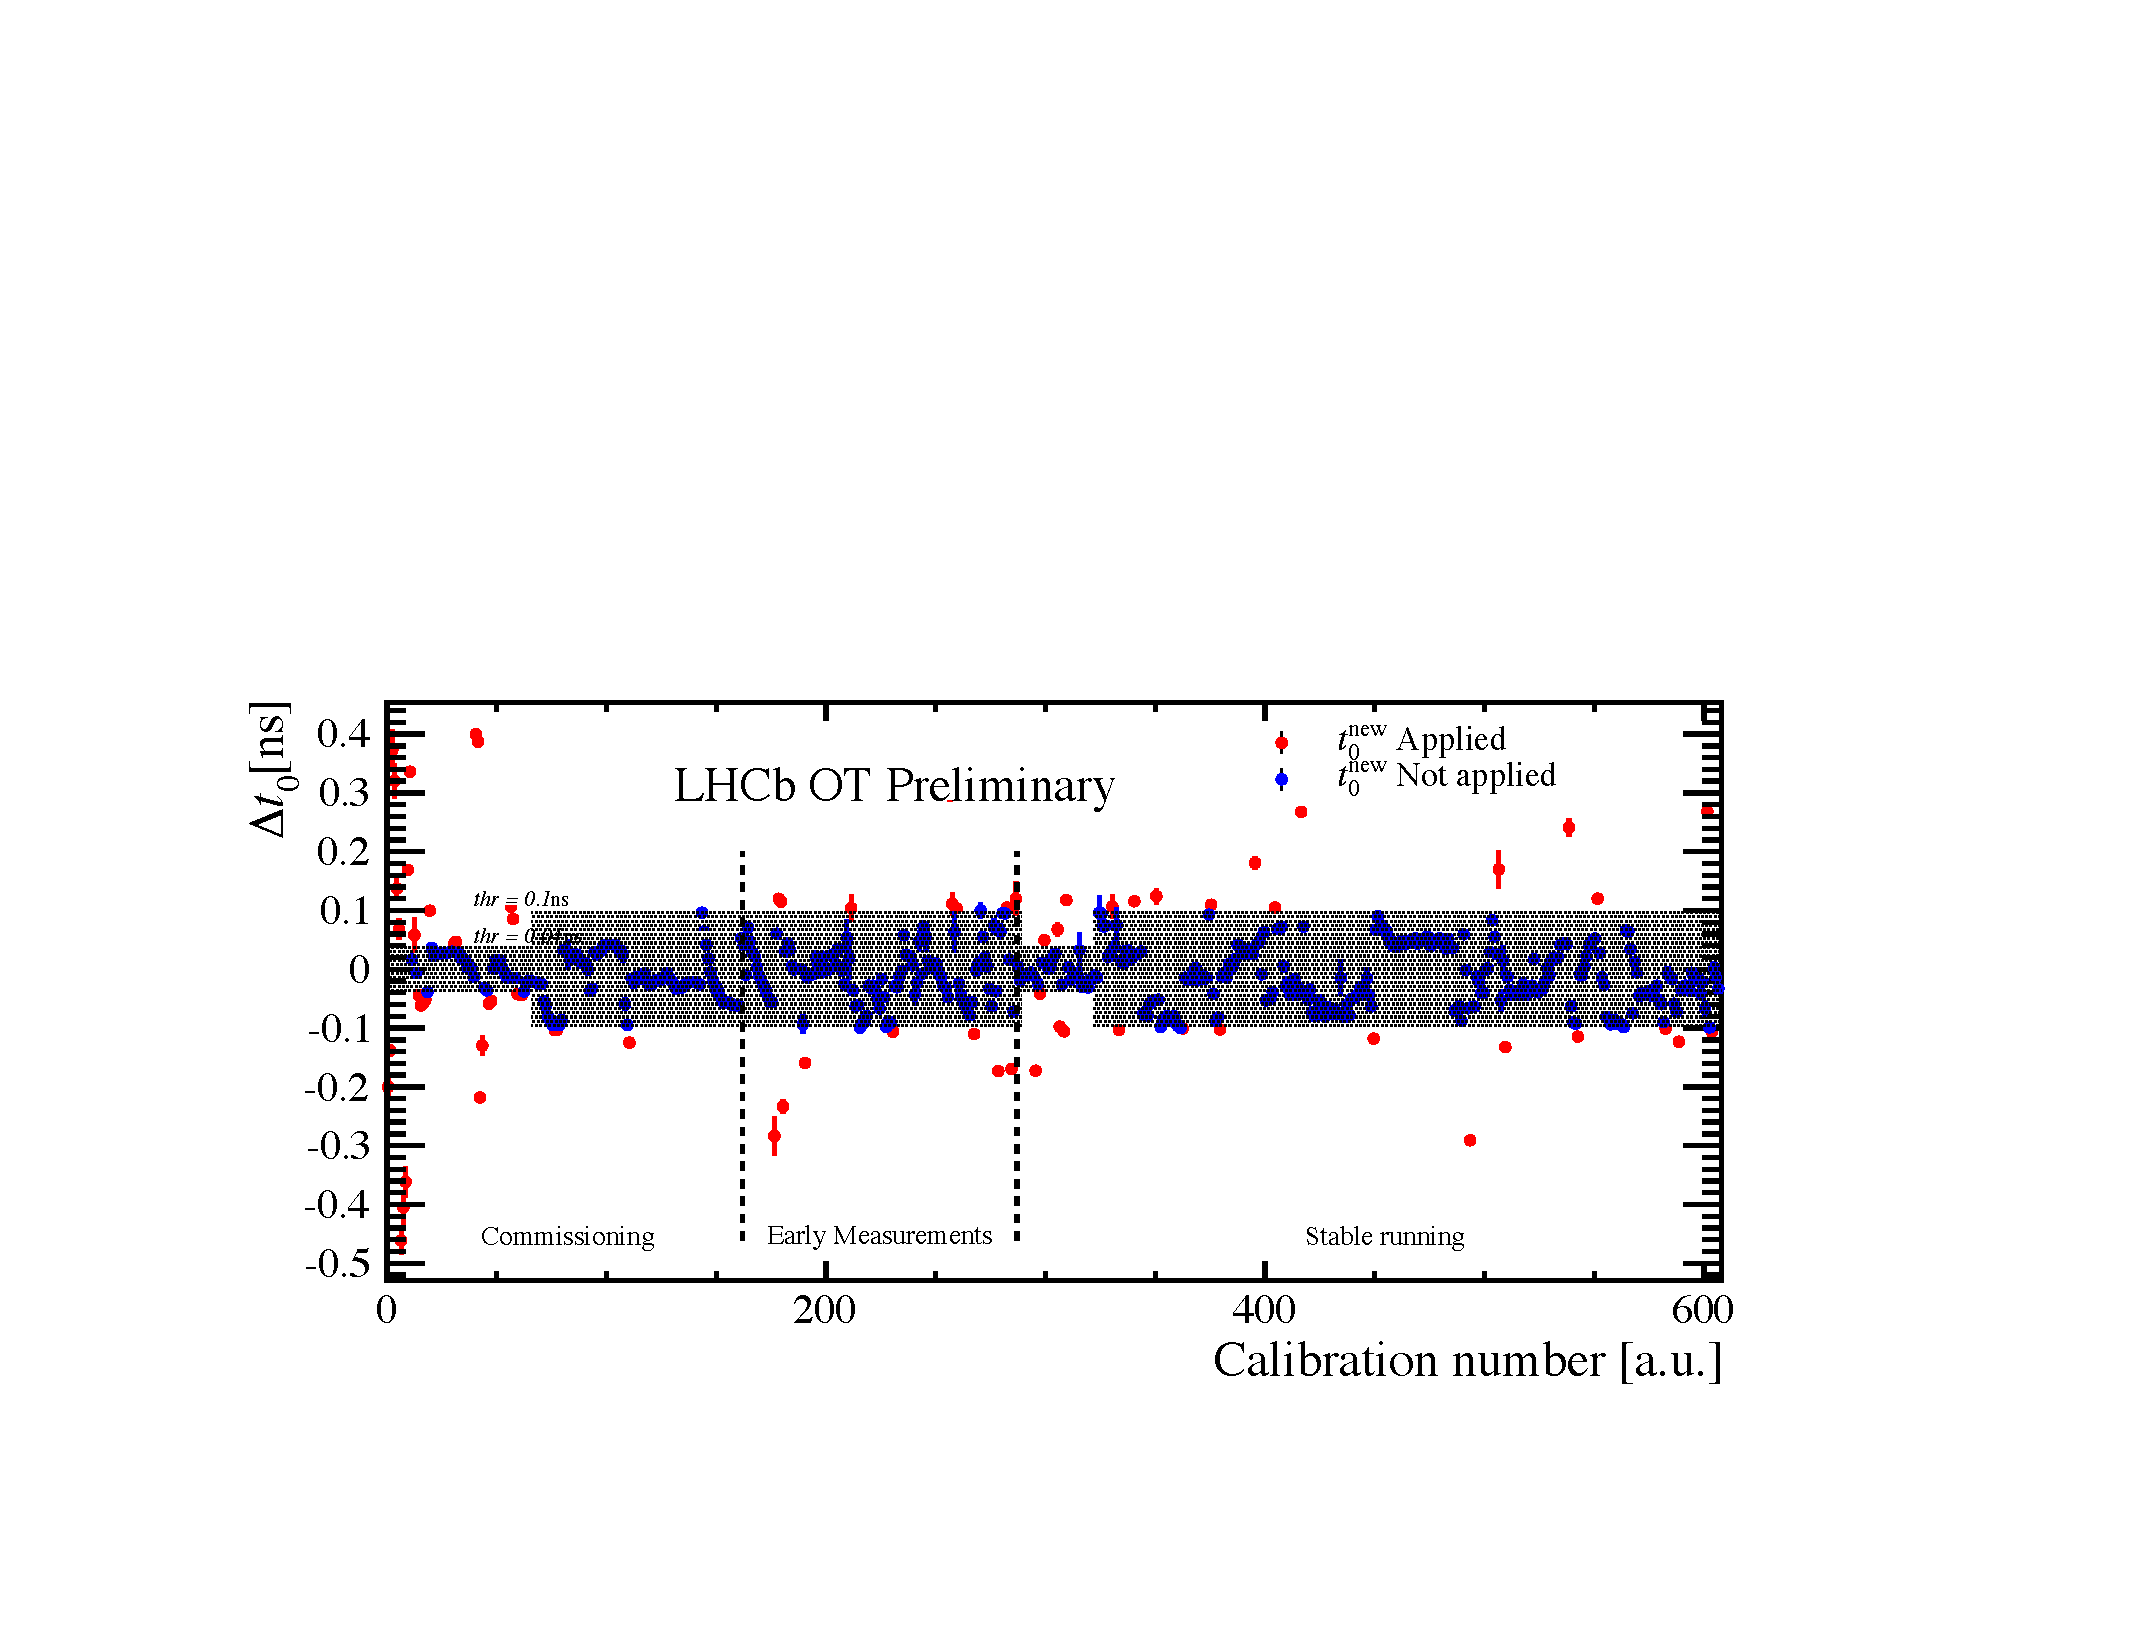
\includegraphics[width=10cm]{../figures/OTt0calibration2015}
  \caption{Global $t_0$ values obtained by the calibration task over time. Red
    points indicate values that were above threshold and therefore propagated to
    online and offline tasks and databases.}
  \label{fig:OT_calib_time}
\end{figure}


\subsection{Calorimeter Calibration}
In order to have a constant L0 rate the calorimeter gain should not
change with time.
The variation of the gain can be estimated by the variation of the
relative occupancy. The occupancy for a cell is defined as the fraction of events in which
the ADC output is above a  threshold. The ratio of the occupancies with respect to a
reference sample is proportional to the changes in gain.
A relative calibration is performed online on a single node for each fill using this occupancy
method and when needed the high voltage is changed accordingly. 

An absolute calibration can be obtained with the $\pi^0$ method: the
reconstructed $\pi^0$ mass can be determined for each cell by fitting di-photon
mass distributions where one of the photon has the cell as the seed. The
calibration coefficients can be tuned to constrain the reconstructed $\pi^0$ mass
 to the nominal one. This fine calibration requires an iterative procedure and
 it is run on the HLT farm similarly to the tracking or RICH mirror alignment. 
This second method takes several hours to run and will be
performed a few times per year i.e. during technical stops.

\subsubsection{Calibration with Relative Occupancy and LEDs}

\begin{figure}[h]
\begin{minipage}{0.5\columnwidth}
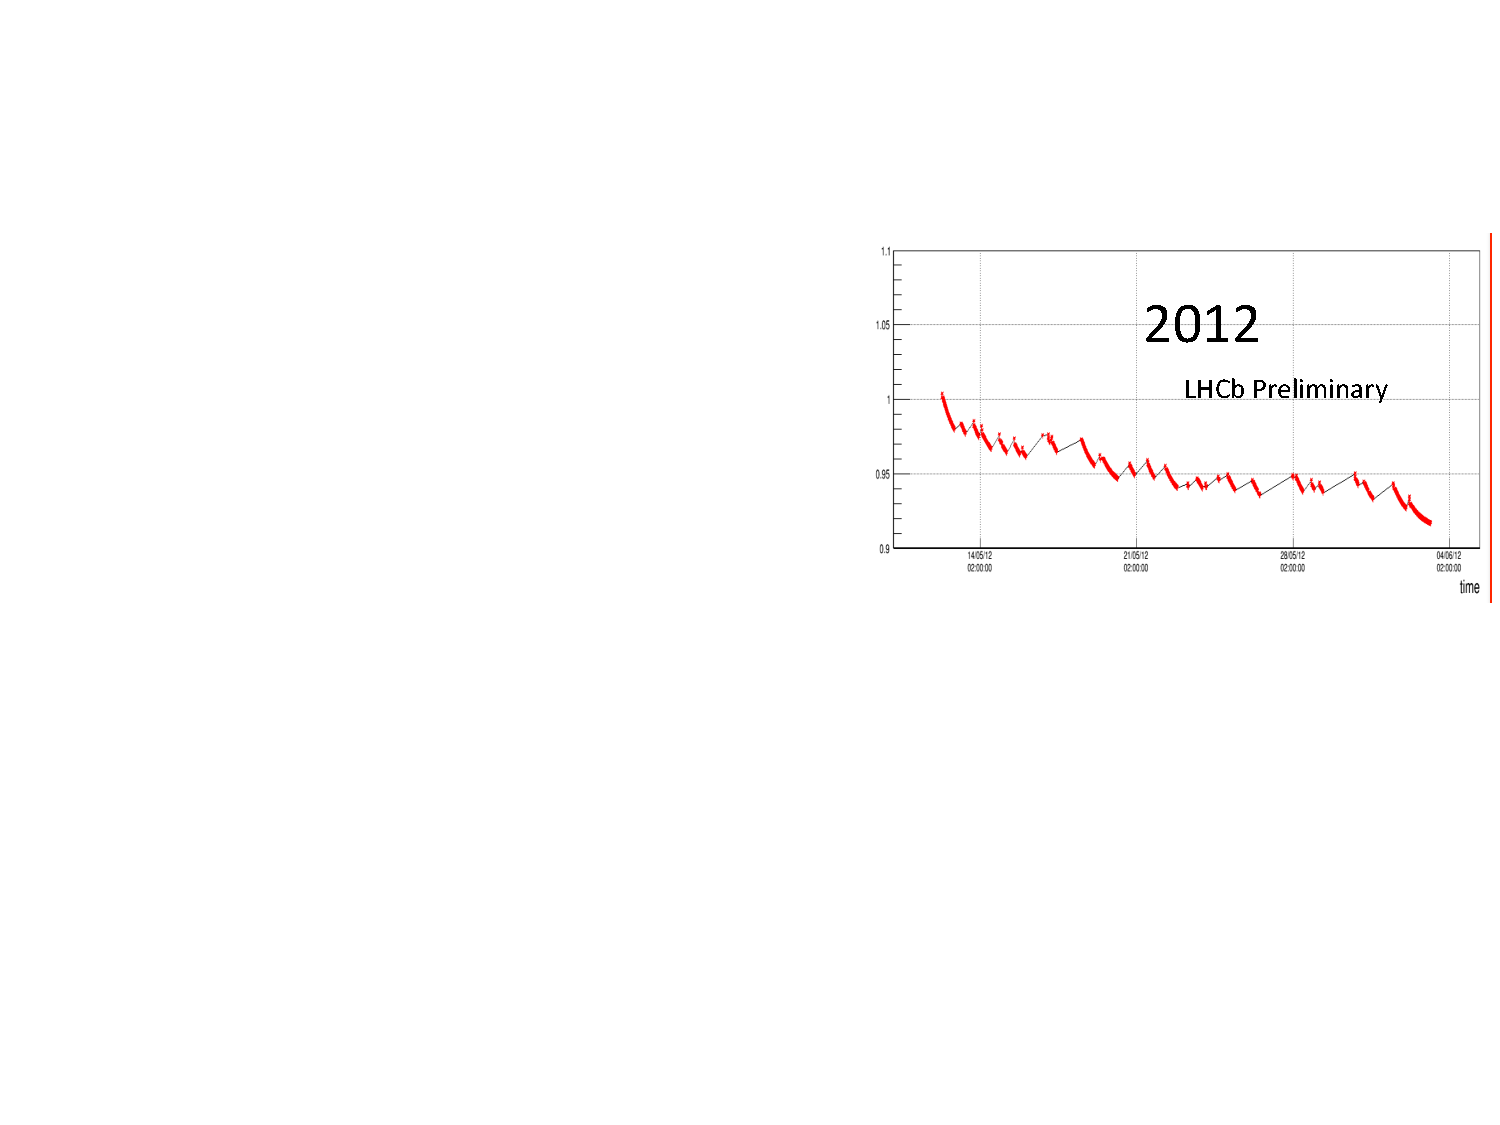
\includegraphics[width=\columnwidth]{../figures/CaloStability2012}
\end{minipage}\hspace{2pc}%
\begin{minipage}{0.5\columnwidth}
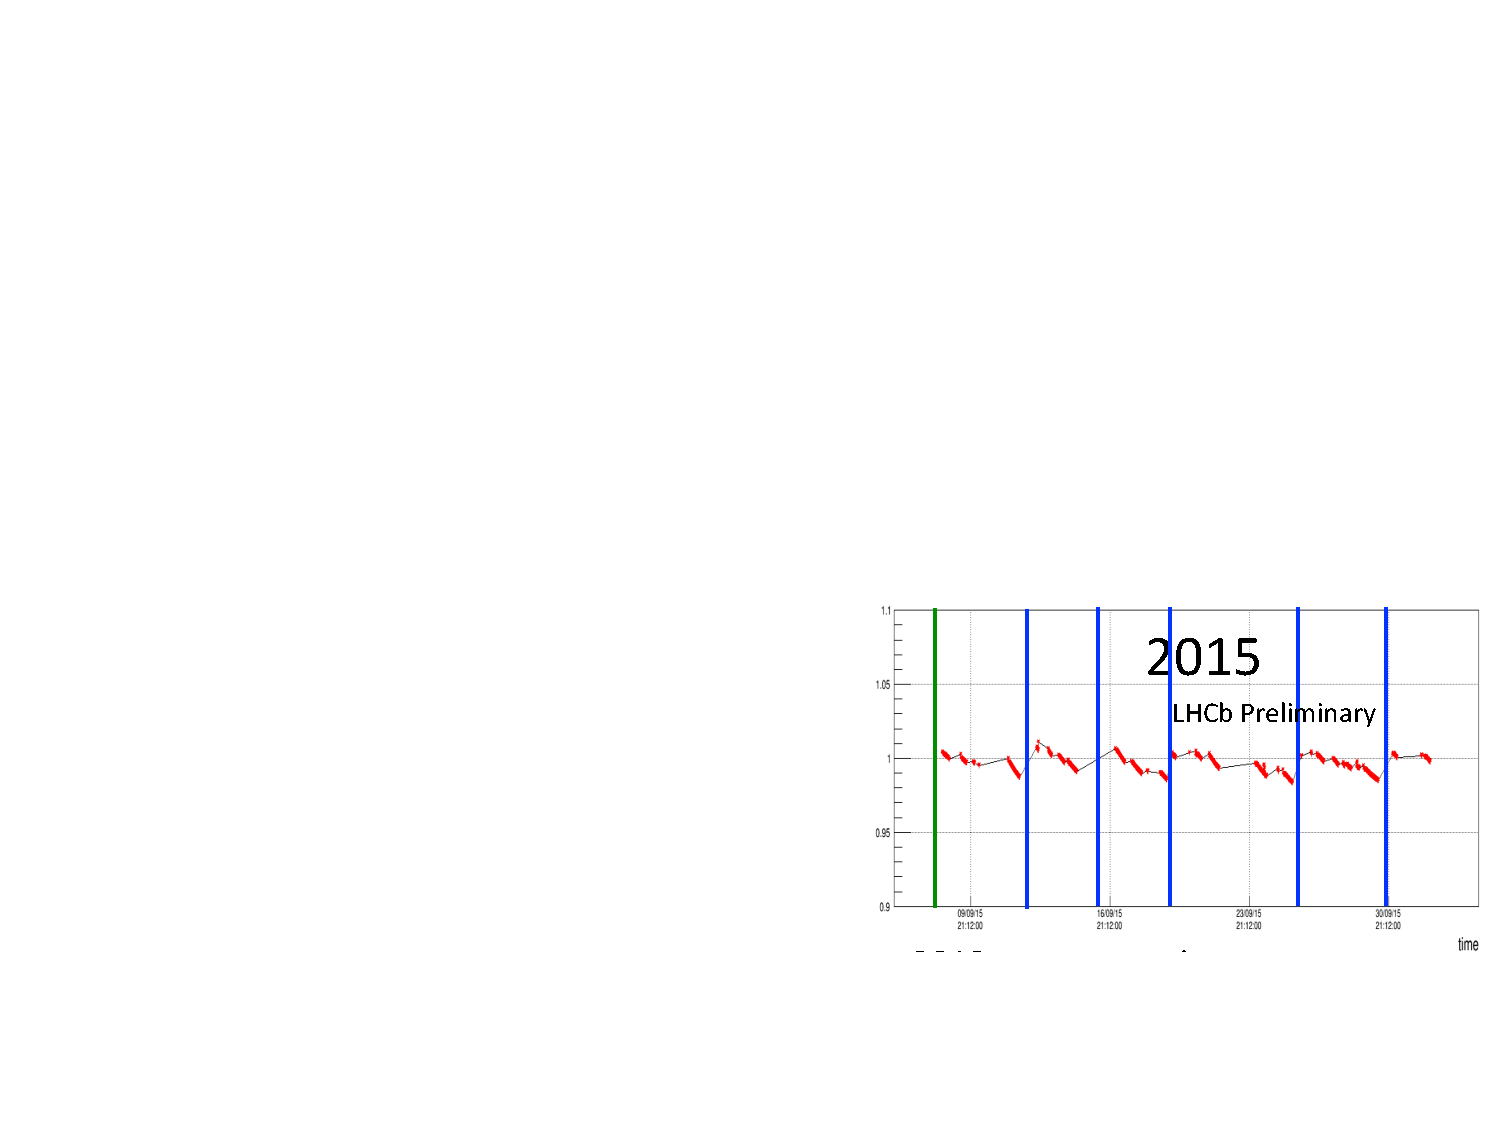
\includegraphics[width=\columnwidth]{../figures/CaloStability2015}
\end{minipage} 
\caption{\label{fig:CaloStability} Stability of calorimeter calibration. Caption to be written, 1st draft for the plot}
\end{figure}

\subsubsection{Absolute Calibration for HCAL with Cs source}


\subsubsection{Absolute Calibration for ECAL with \texorpdfstring{\piz}{pi0}}

\begin{figure}[h]
  \centering
  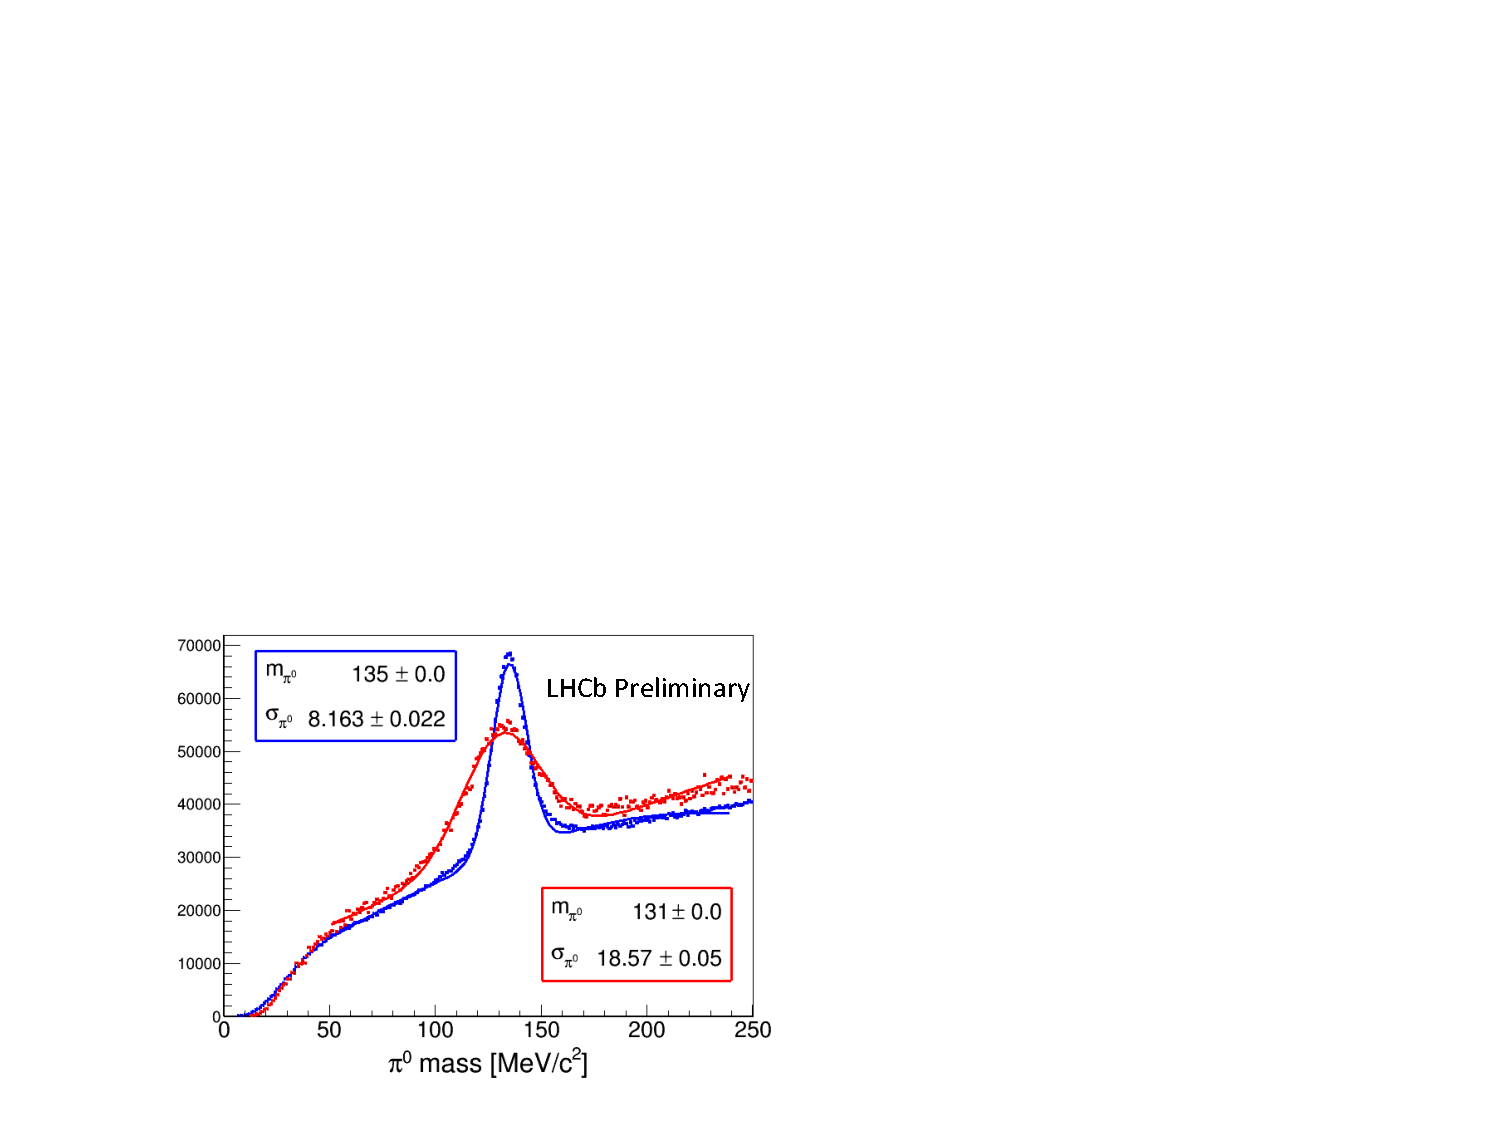
\includegraphics[width=8cm]{../figures/CaloPi0Calibration2015}
  \caption{ Stability of calorimeter calibration. Caption to be written, 1st draft for the plot}
  \label{fig:Calo_Pi0calib}
\end{figure}







\section{Scheduling}
\textcolor{red}{ Give an overview of the scheduling for all the tasks: at beginning of each fill? each 1 week?
when we update constants/hv/ if trigger run change. Some details could/should included in each section but probably it would be good to have some `overview' of the schedule.}


\section{Propagation of Constants}

\begin{table}
\begin{tabular}{l l}
  Task                  & Used by                 \\ \hline
  Velo alignment        & HLT1, HLT2 and offline  \\ 
  tracker alignment     & HLT1, HLT2 and offline  \\
  muon alignment        & L0 Muon and monitoring  \\
  ECAL calibration      & update of ECAL high voltages \\
  RICH mirror alignment & HLT2 and offline        \\
  RICH calibrations     & HLT2 and offline        \\
  OT calibration        & HLT1, HLT2 and offline
\end{tabular}
\caption{Processing phases or detector systems that require the result of
  calibration and alignment tasks.}
\label{tab:results_needed}
\end{table}

Once a calibration or alignment task has completed, it writes the constants it
produced to one or more XML file. To allow propagation of these constants to the
data processing tasks, such tasks have been configured to read relevant
calibration and alignment constants from these XML files. Whenever a task
receives an event that belongs to a new data taking period, a new set of XML
files is read to obtain the latest constants. 

\Cref{tab:results_needed} gives on overview of where constants are used. The
different phases where constants are needed broadly fall into three categories:
HLT1, HLT2 and offline; HLT2 and offline; and detector subsystems. If constants
are used in HLT1, HLT2 and offline, they are used across all of these phases
starting from a fixed point in time after the result has been obtained. This
usually means the start of the next data-taking period of up to an hour. If
constants are not needed in HLT1, but only by HLT2 and offline, HLT2 will not
start processing data from a given data-taking period until the constants for
that data-taking period have been produced. Results of tasks used only by
subsystems are interpreted by subsystem experts and used to make updates to the
configuration of those system if and when required.

If constants are needed for offline processing, they are added to the
conditions database as soon as all constants for a given data taking period are
available. Once the constants have been added to the conditions database, a
cross-check is performed by configuring one task to read the constants from the
XML files, another task to read them from the conditions database, and comparing
the constants they obtain. If any mismatches are detected, the corresponding
data taking period is not declared ready for offline processing. Experts then
investigate the source of the mismatches and resolve the problem.


\section{Benefits to Physics}
textcolor{red}{maybe here more on trigger efficiency or put here high level quantity like mass or time or pid..... to be decided. When the different sections are ready we can decide if we want to move some performance in this section.\\

How this reflects in "physics" (comparison run1/run2 or with/without the update alignment/calibration) \\
for example the rate of the D->Kpipipi \\
stability of mass plot? or PV resolution? or proper time/ip chi2/ ip? \\
systematic? due to online/offline difference or alignment variation (efficiency or ip selection or difference acceptance online/offline)
}


\section{Conclusion}
In Run~II the new scheme for the software trigger at LHCb allows the
alignment and calibration to be performed in real time. A dedicated framework
has been put in place to parallelise the alignment and calibration tasks
on the multi-core farm infrastructure used for the trigger in order to meet the
computing time constraints. Data collected
at the start of the fill are processed in a few minutes and the output is used to
update the alignment, while the RICH calibration constants are evaluated for
each run. The same framework is used to perform  finer calibration less
frequently and to monitor the alignment quality of various subdetector. 
This procedure allows a
more stable alignment quality, more effective trigger selections and
online-offline consistency thanks also to the same online-offline reconstruction.
Physics analysis can be performed directly on the trigger output with the same online-offline performance.



% Do not include this in analysis note and conference reports
\section*{Acknowledgements}

The text below are the acknowledgements as approved by the collaboration
board. Extending the acknowledgements to include individuals from outside the
collaboration who have contributed to the analysis should be approved by the
EB. The extra acknowledgements are normally placed before the standard 
acknowledgements, unless it matches better with the text of the standard 
acknowledgements to put them elsewhere.
They should be included in the draft of first circulation.
 
\noindent We express our gratitude to our colleagues in the CERN
accelerator departments for the excellent performance of the LHC. We
thank the technical and administrative staff at the LHCb
institutes. We acknowledge support from CERN and from the national
agencies: CAPES, CNPq, FAPERJ and FINEP (Brazil); NSFC (China);
CNRS/IN2P3 (France); BMBF, DFG, HGF and MPG (Germany); INFN (Italy); 
FOM and NWO (The Netherlands); MNiSW and NCN (Poland); MEN/IFA (Romania); 
MinES and FANO (Russia); MinECo (Spain); SNSF and SER (Switzerland); 
NASU (Ukraine); STFC (United Kingdom); NSF (USA).
The Tier1 computing centres are supported by IN2P3 (France), KIT and BMBF 
(Germany), INFN (Italy), NWO and SURF (The Netherlands), PIC (Spain), GridPP 
(United Kingdom).
We are indebted to the communities behind the multiple open 
source software packages on which we depend. We are also thankful for the 
computing resources and the access to software R\&D tools provided by Yandex LLC (Russia).
Individual groups or members have received support from 
EPLANET, Marie Sk\l{}odowska-Curie Actions and ERC (European Union), 
Conseil g\'{e}n\'{e}ral de Haute-Savoie, Labex ENIGMASS and OCEVU, 
R\'{e}gion Auvergne (France), RFBR (Russia), XuntaGal and GENCAT (Spain), Royal Society and Royal
Commission for the Exhibition of 1851 (United Kingdom).


% This should be taken out in the final paper
\addcontentsline{toc}{section}{References}
\setboolean{inbibliography}{true}
\bibliographystyle{LHCb}
\bibliography{main,LHCb-PAPER,LHCb-CONF,LHCb-DP,LHCb-TDR}


\newpage
\end{document}
